\chapter{Detector commissioning}
\label{ch:commissioning}

The commissioning of the SuperNEMO demonstrator has begun in $2019$ and first calorimeter data was taken.\\
The calorimeter of SuperNEMO is segmented in $712$ optical modules (OM), each composed by a coupling between a photomultiplier tube (PMT) and a polystyrene scintillator bloc (see Sec.~\ref{sec:calorimeter} for more details).
The divider of a PMT is connected to $2$ cables, one providing the high voltage (HV), the other one, called signal cable, is a coaxial cable collecting and transporting the charge provided by the PMT.\\
By the summer $2020$, the SuperNEMO demonstrator will be encapsulated in an anti radon tent.
The so called \emph{patch panel} will insure passage of cables from the inside, to the outside of the anti radon tent, therefore doubling the amount of cables needed for the calorimeter.
We refer to the cables running from detector to patch panel as \emph{internal} cables, and the cables from patch panel to the electronic boards as \emph{external} cables.
Consequently, regarding only the calorimeter part, 2848 cables were cut, assembled, connector-mounted, transported and installed at LSM.
Then the check of every cable condition is mandatory to control and eventually fix them.

\section{Reflectometry analysis}
\label{sec:reflecto}

\subsection{Goal of the reflectometry analysis}

Taking into account the final demonstrator design, each coaxial length was determined, cables were cut and labelled in LAL, Orsay.
All external coaxial cables were designed to be $7$ meters-long -- the distance between electronic boards and patch panel being the same for all channels at electronic boards -- and internal cable lengths have been adapted to fit the distance from the patch panel to each optical module.
Then, cutting and labelling all cables lasted several weeks.
After all cables were transported and installed at LSM, we had to check each coaxial cable condition, for several reasons:
\begin{itemize*}
\item check if no cable was damaged during the transport and the installation;
\item control if no swap between cables has been made during cable labelling or calorimeter cabling,
\item check if the coaxial cable was cut at the right length,
\item more importantly estimate the signal time delay due to the cable lengths: knowing that the velocity of electrons in the coaxial cables has a known constant value, the longer is the cable, the more the signal takes time to travel from the PMT to the electronic channel.
  Therefore, each coaxial cable length has to be characterised, especially if we want to do time coincidences between two signals in two different channels.
\end{itemize*}
To do so, a pulse, called \emph{primary} pulse, is generated at the electronic board readout.
The signal will travel all along the coaxial cable, from the electronic board to the PMT divider.
Whether the cable is correctly connected to the PMT or not, the signal reflects at the other end.
\begin{figure}[h]
  \centering
  \begin{subfigure}[b]{0.3\textwidth}
    \centering
    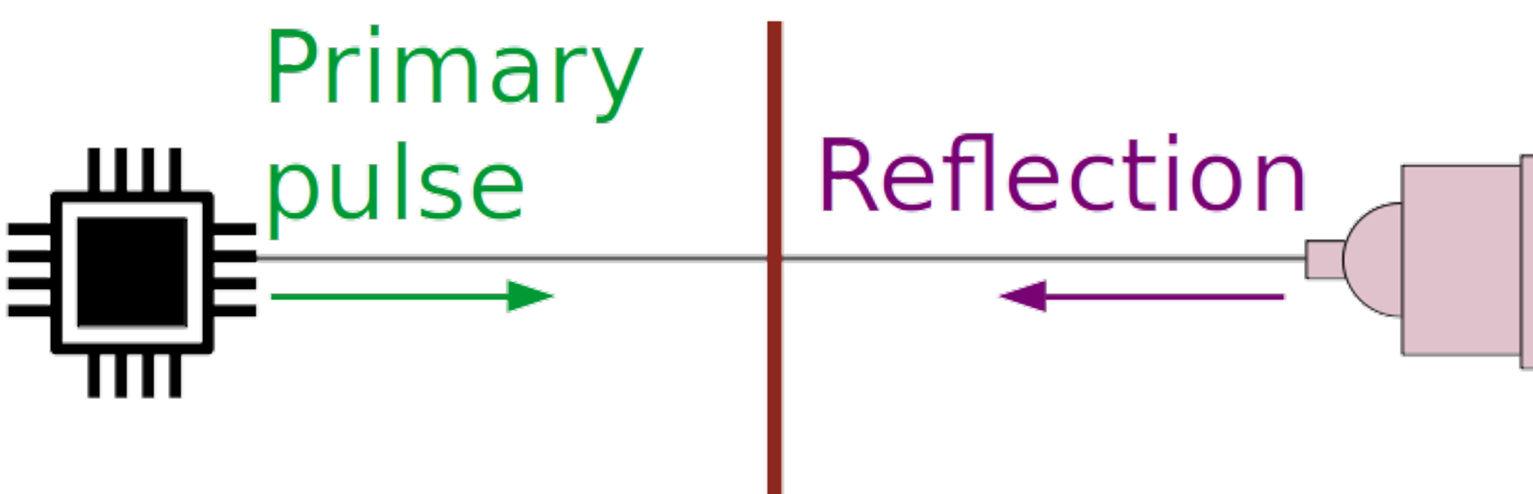
\includegraphics[width=1.1\textwidth]{commissioning/fig_commissioning/scheme_reflecto.pdf}
    \captionsetup{justification=centering}
    \caption{Normal reflection at PMT divider.
      \label{subfig:reflecto_normal}}

  \end{subfigure}
  \hfill
  \begin{subfigure}[b]{0.3\textwidth}
    \centering
    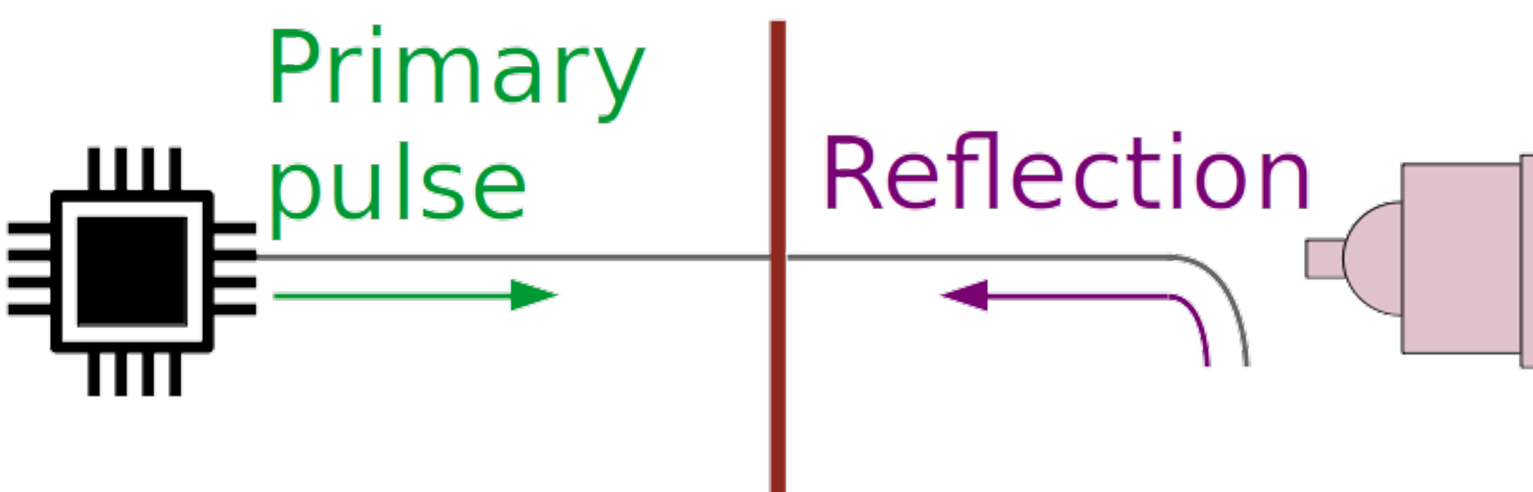
\includegraphics[width=1.1\textwidth]{commissioning/fig_commissioning/scheme_reflecto_1.pdf}
    \captionsetup{justification=centering}
    \caption{Cable not connected at PMT.
      \label{subfig:reflecto_pmt}}

  \end{subfigure}
  \hfill
  \begin{subfigure}[b]{0.3\textwidth}
    \centering
    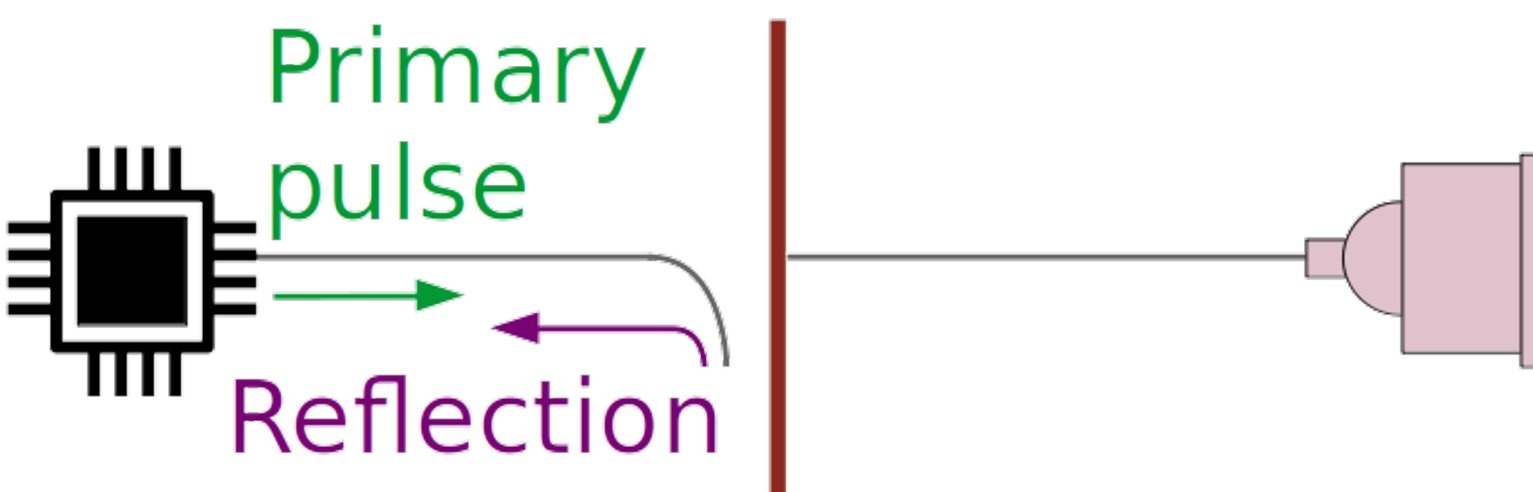
\includegraphics[width=1.1\textwidth]{commissioning/fig_commissioning/scheme_reflecto_2.pdf}
    \captionsetup{justification=centering}
    \caption{Cable not connected at patch panel.
      \label{subfig:reflecto_pp}}

  \end{subfigure}
  \caption{A representation of pulses sent in a cable for the reflectometry analysis is given.
    The electronic boards are symbolised by the black chip, and the patch panel by the red vertical bar.
    Three scenario where a primary pulse is sent in one cable (represented in grey), are represented.
    (a) The cable is well connected at the patch panel and at the PMT. The signal reflects at the PMT divider.
    (b) The cable is not connected at PMT and the signal is reflected at the end of the cable.
    (c) The cable is not connected at patch panel and the signal is reflected at the end of the external cable.\label{fig:reflecto_scheme}}

\end{figure}
Then the signal travels back from the PMT to the electronic board channel, where it is recorded by the acquisition.
We called this recorded reflected pulse \emph{secondary} pulse.
An example of the total recorded signal is displayed in Fig.~\ref{subfig:total_waveform}.
In order to accumulate enough statistics, we send thousands of pulses in each coaxial cable.
The analyses of the shape and of the arrival time of those secondary pulses for each channel is called \emph{reflectometry}, and allow us to check the coaxial cable conditions and to control their lengths.

\subsection{Pulse timing: controlling cable lengths}
\label{subsec:timing}

The first step of this analysis is to experimentally determine the length $l_{j}^{m}$ for all signal cables $j$ installed on the demonstrator.
This length is defined as
\begin{equation}
  l_{j}^{m}= 0.5\,t_{j}\,v_{p}\, ,
\end{equation}
where $t_{j}$ stands as the time made by the electrons to do a round trip between one electronic channel and one PMT, and $v_{p}$ is the velocity of electrons in the coaxial cables, which can be expressed as a fraction of light speed in vacuum, $c$.
The time difference $t_{j}$ between the primary pulse and the secondary pulse is written as
\begin{equation}
  t_{j} = \braket{t_{\text{secondary pulse}}-t_{\text{primary pulse}}}_{p} \, \text{,}
\end{equation}
$\braket{}_{p}$ being the average over all pulses sent in one single cable $j$.
The velocity $v_{p}$ is supplied by the cable manufacturer as
\begin{equation*}
  v_{p}=\frac{c}{\sqrt{\epsilon_{r}}}\,\text{,}
\end{equation*}
with $\epsilon_{r}$ the relative dielectric constant of the material.
Therefore, this celerity depends on the components.
For the coaxial cables chosen in the demonstrator design, the data sheet of the cable gives ${v_{p}=0.69\,c}$.
A study is performed to verify experimentally the value of $v_{p}$.
Three cables of different lengths are measured with a precision of $1$ cm.
A thousand of primary pulses are sent in each of the three cables, then the time for each secondary pulse is recorded.
At the end, we have three independent measures of the velocity $v_{p}$ in the used coaxial cables.
In Fig.~\ref{fig:celerity} is displayed the lengths $l_{j}$ as a function of the times $t_{j}$.
\begin{figure}[h]
  \centering
  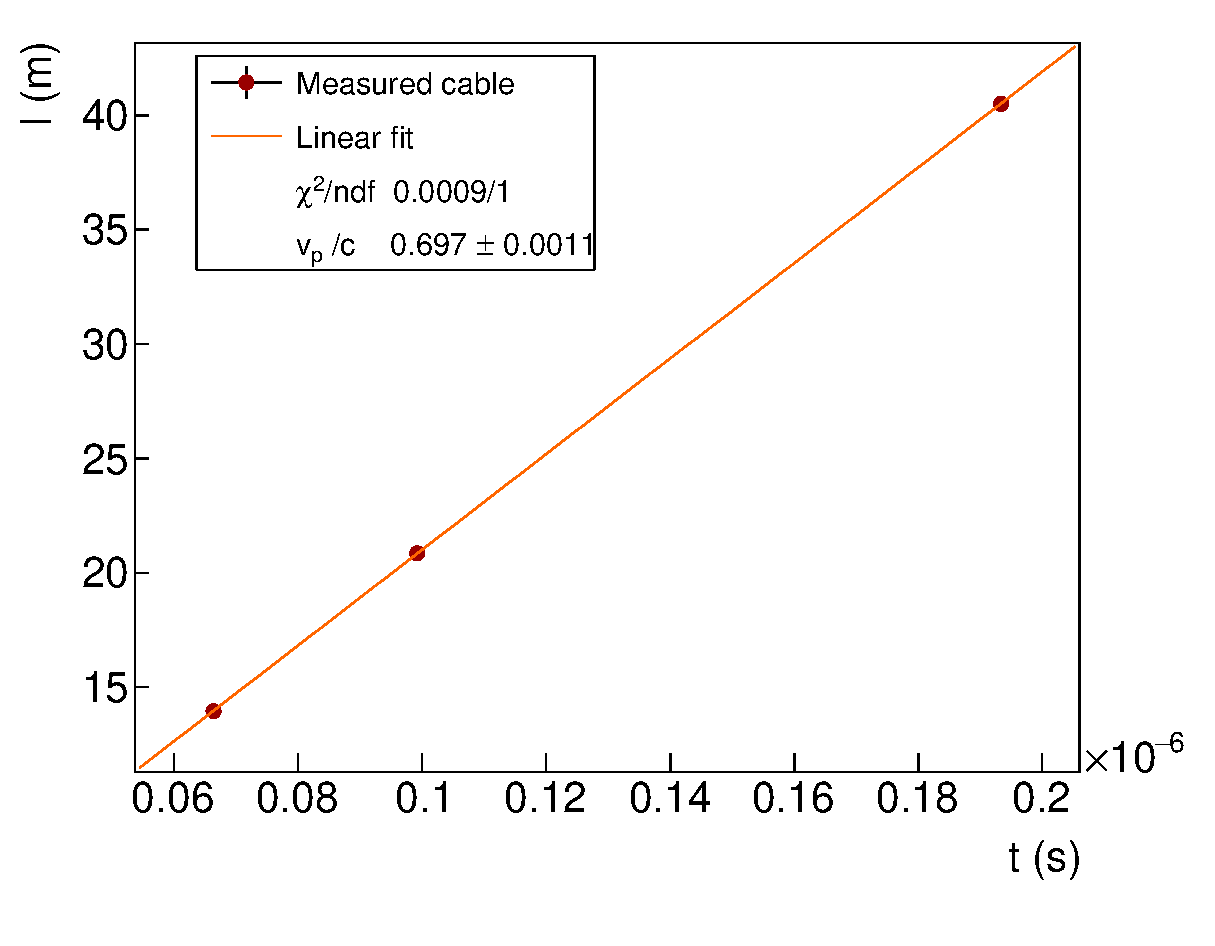
\includegraphics[width=15cm]{commissioning/fig_commissioning/celerity.eps}
  \caption{Three different lengths $l_{j}$ of cables are measured.
    Pulses are sent inside all cables.
    The lengths $l_{j}$ are plotted as a function of the time differences $t_{j}$ between primary and secondary pulses.
    The value of $v_{p}/c$ fitted from the data points is displayed.
    This value of $0.697\pm 0.0011$ shows the compatibility with the one supplied by the constructor, of $0.69$ c.
    \label{fig:celerity}}
\end{figure}
The fitted value of $v_{p}/c = 0.697\pm 0.0011$ is displayed and shows a compatibility up to $7\sigma$ with the data sheet.

As we want to determine the time interval $t_{j}$, we have to define what is the \emph{time} of a pulse.
In this analysis, we use a technique called Constant Fraction Discriminator (CFD), providing an amplitude-independent information about time of a pulse.
This algorithm aims at tracking a signal and defining its time arrival at a given fraction $f$ of its maximal amplitude.
The two main advantages of this technique is that it provides an efficient rejection of the noise in the acquisition window, and gives a good resolution on the measured time.
Nevertheless, the possible influence of the chosen value for the $f$ parameter on this time resolution has to be investigated.
We perform such a study in Sec.~\ref{subsec:CFD}.
We concluded that the highest precision on the time measurement arises for $f = 40\%$, and we adopt this value for the following analysis.
A graphic representation of the CFD time search is given in fig.~\ref{subfig:zoom_secondary}.
\begin{figure}[h]
  \centering
  \begin{subfigure}[t]{0.7\textwidth}
    \centering
    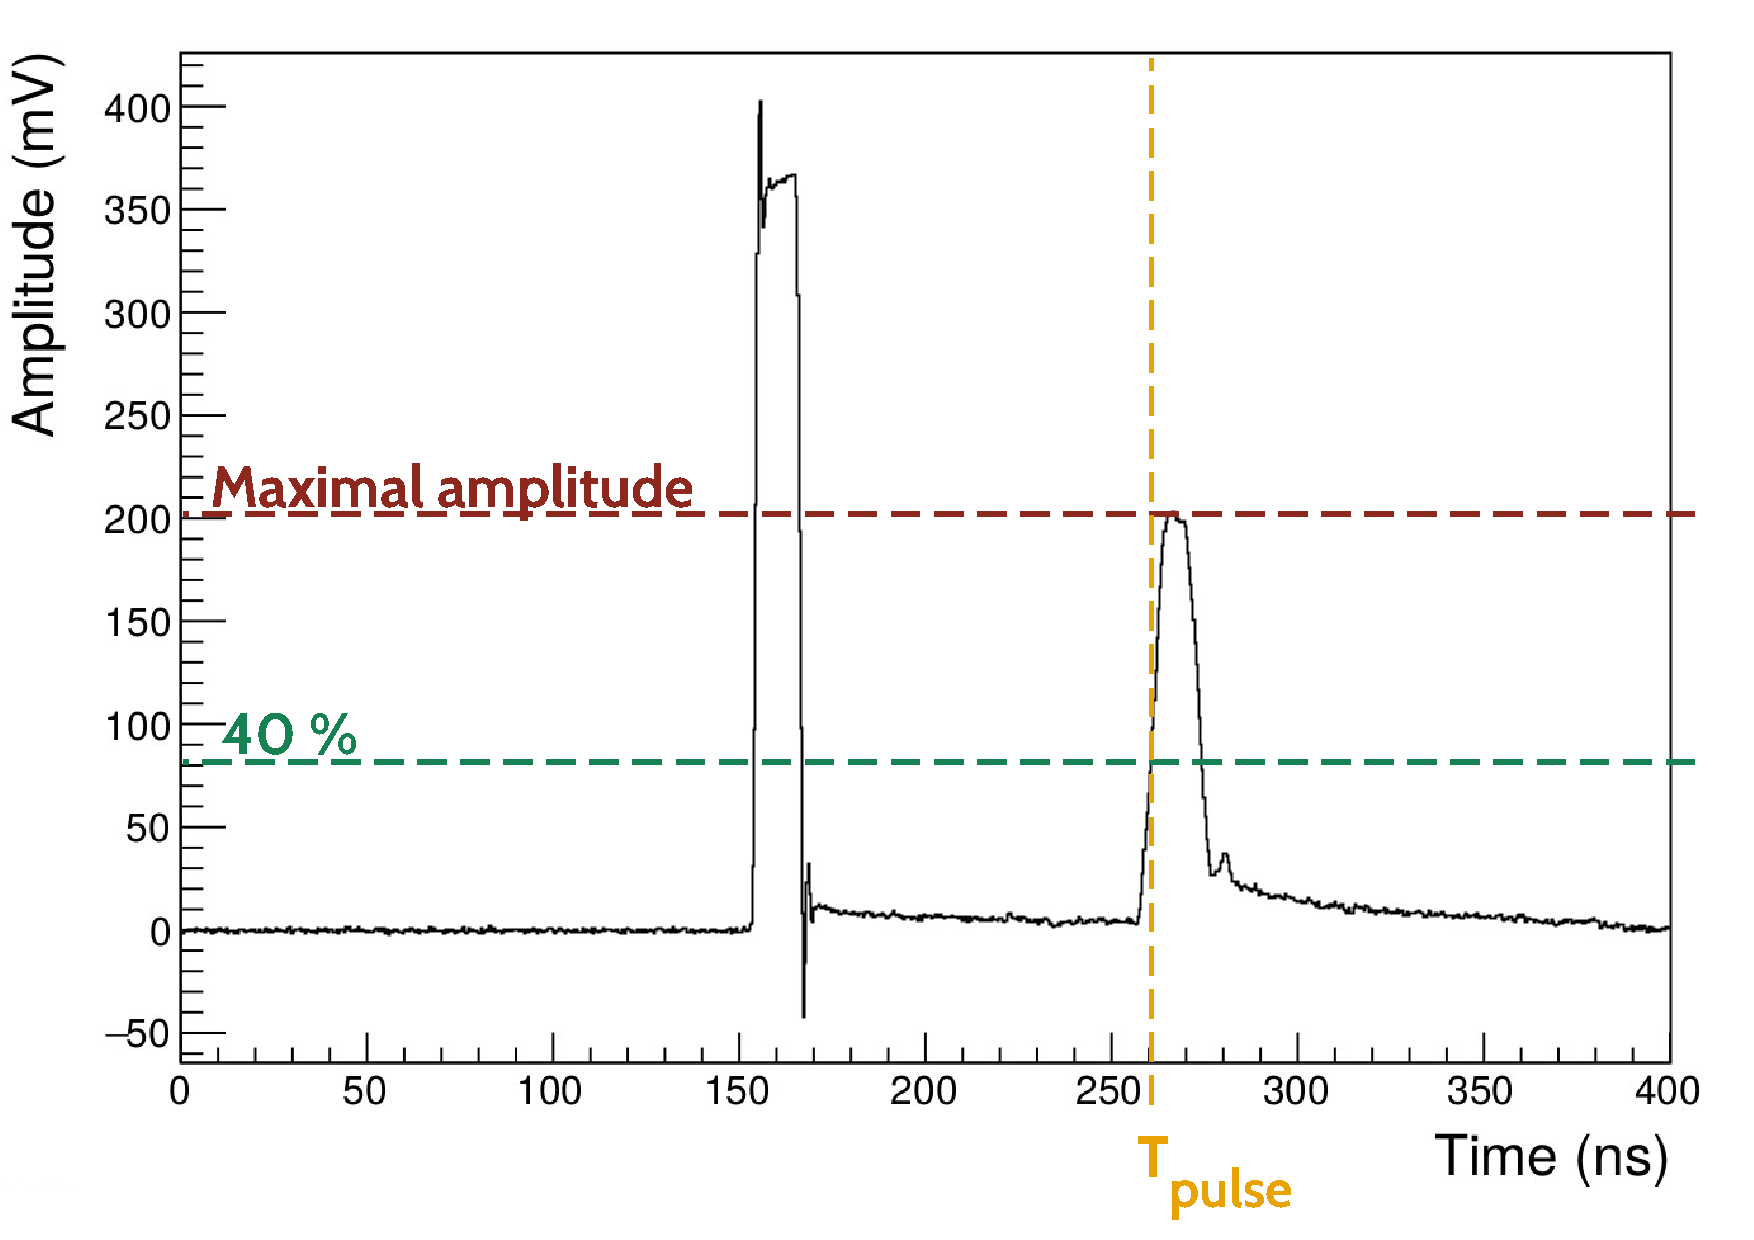
\includegraphics[trim={1.2cm 3.5cm 1.7cm 3.1cm},clip,width=1\textwidth]{commissioning/fig_commissioning/CFD_example.pdf}
    \captionsetup{justification=centering}
    \caption{Total recorded waveform
      \label{subfig:total_waveform}}
  \end{subfigure}
  \hfill
  \begin{subfigure}[t]{0.7\textwidth}
    \centering
    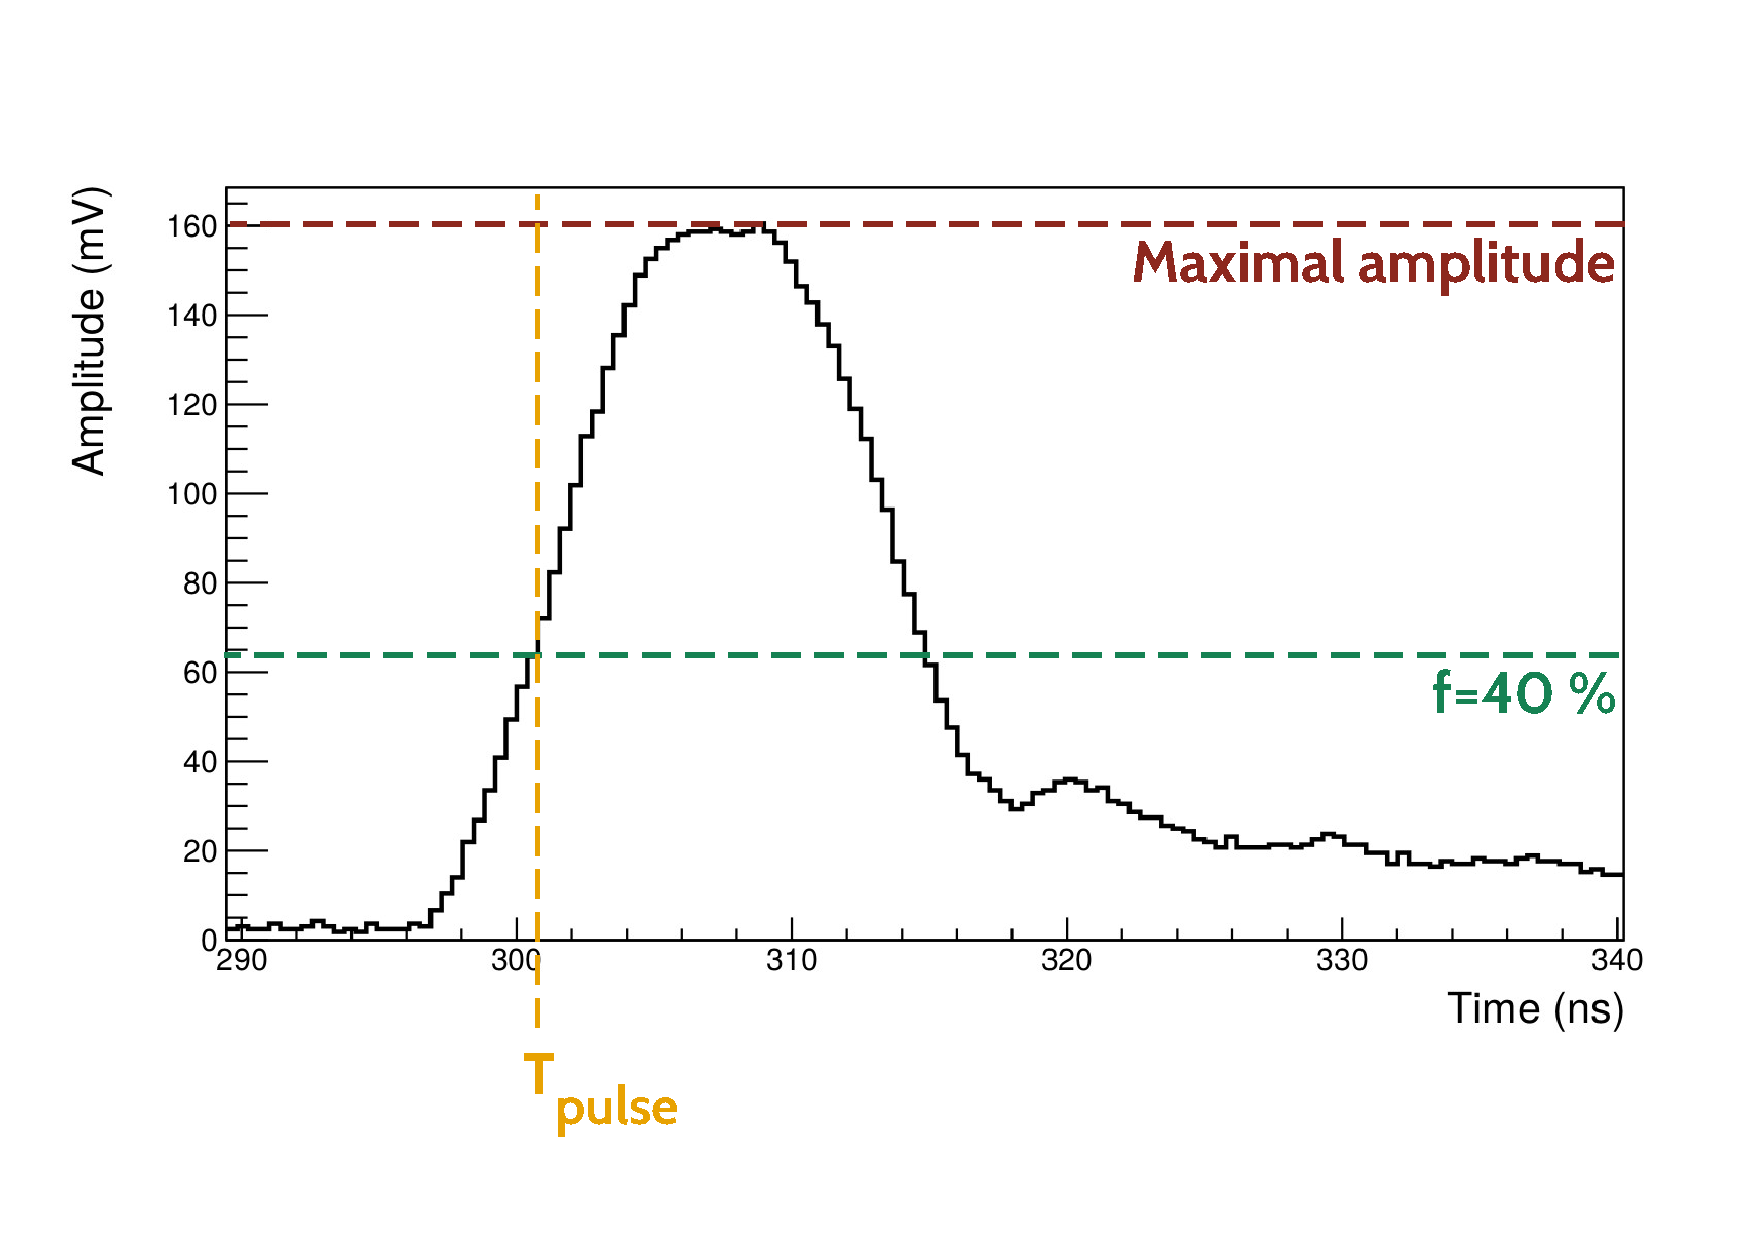
\includegraphics[trim={1.2cm 1.5cm 1.7cm 3.1cm},clip,width=1\textwidth]{commissioning/fig_commissioning/CFD_example_zoom.pdf}
    \captionsetup{justification=centering}
    \caption{Zoom on secondary pulse
      \label{subfig:zoom_secondary}}
  \end{subfigure}
  \caption{(a) Total recorded waveform: primary pulse (left) and secondary the pulse (right).
    (b) Zoom on the secondary pulse.
    A representation of time computed with a Constant Fraction Discriminator (CFD) is provided.
    Its maximal amplitude (red dotted line) and its fraction for $\text{f}=40\%$ (green dotted line) are displayed.
    The time $\text{T}_{\text{pulse}}$ (orange dotted line) represents the time of arrival of the secondary pulse computed with CFD, with the fraction $\text{f}=40\%$.
    \label{fig:CFD}}
\end{figure}
As we want to measure the installed cable lengths $l^{m}_{j}$, and compare them to the initially designed ones, $l^{d}_{j}$, we define the length difference $\Delta L_{j}$ as:
\begin{equation}
  \Delta L_{j} = l^{m}_{j}-l^{d}_{j}\, .
\end{equation}
In Fig.~\ref{fig:LengthDiff} is displayed the distribution $\Delta L$ for all the measured lengths.
\begin{figure}[h]
  \centering
  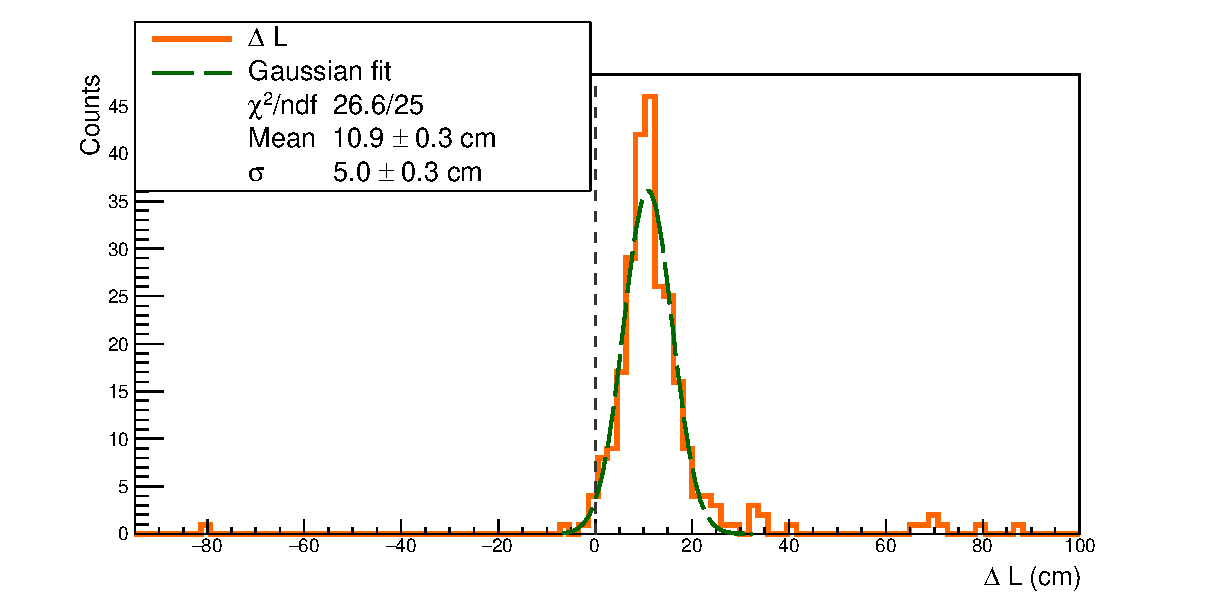
\includegraphics[width=15cm]{commissioning/fig_commissioning/length_diff.eps}

  \caption{The distribution of difference between the measured lengths $l^{m}$ and the expected lengths $l^{d}$ is displayed in orange solid line.
    The black dashed line represents the case where $l^{m}_{j} = l^{d}_{j} \;\forall j$.
    The Gaussian fit (green dashed line) presents a mean of $10.9 \pm 0.3$ cm.
    Some data points considered as outliers are beyond $3\sigma$.
    \label{fig:LengthDiff}}
\end{figure}
In hypothetical perfect conditions, all the cables should fit the design length, in other words, $l^{d}_{j} = l^{m}_{j}$.
Consequently the $\Delta L$ distribution should a peak at zero, as materialised by the black dashed line.
However, in real conditions, the measured length can be different from the designed one, leading the $\Delta L$ distribution plotted in orange solid line.
We conclude that the observed cable length $l^{m}$ differs from $l^{d}$ by $+10.9\pm 0.3$ cm, meaning that cables are longer than expected in average.
This may reveal a bias coming from the device used to cut the cables.
In fact, during cable cutting work, we noticed that the cutting device had a tendency to slip, probably leading to cables with extra lengths.
We assumed the cutting device has a given probability to slip for one meter of cable.
If this is the case, the probability for the device to give extra length should increase with the cable length.

To verify this assumption, we plot in Fig.~\ref{fig:CutBias} the length difference $\Delta L$ as a function of the initial design length $l^{d}$ (cyan).
From those data points, we compute a linear fit (orange solid line), parameterised as $y = \alpha x + \beta$, revealing that the cutting device presents two different biases.
\begin{figure}[h]
  \centering
  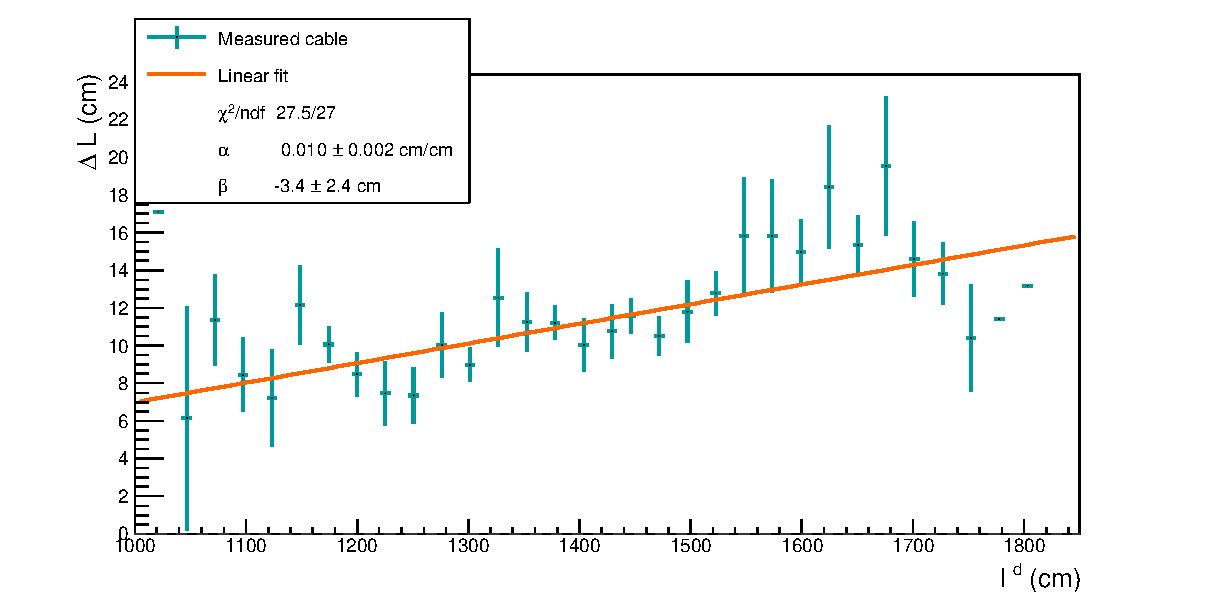
\includegraphics[width=15cm]{commissioning/fig_commissioning/cut_biais.eps}

  \caption{$\Delta L$ is plotted with $l^{d}$ (cyan), where $l^{d}$ is averaged for all the lengths designed to have the same value, being at the origin of vertical error bars.
    In black dashed line is represented the case where $l^{m} = l^{m}$.
    Data points are fitted by $\alpha x + \beta$, with $\alpha > 0$ and $\beta < 0$, revealing the two biases of the cutting device.
    \label{fig:CutBias}}
\end{figure}
The value of $\beta$ shows that the cutting device systematically took away $3.4$ cm of each cable.
Nevertheless, as the shortest cable was designed to be 10 meters long, there are no important consequences of this bias on the length difference $\Delta L$.
Besides, the slope $\alpha = 0.010\pm 0.002$ of the linear fit reveals that the cutting device adds one centimetre for every meter of cable, being compatible with the hypothesis on the cutting device sliding.
Hopefully this bias is not problematic as it makes most of the actual cable lengths longer than the design, while shorter lengths could have lead to systematic connection issues to PMTs.
However, we notice that a few cables have been cut too short by mistake, the worse of them being $80$ centimetres shorter than expected.
Fortunately, this cable  was successfully connected to PMT despite this deficit.
On the contrary, few cables have a large extra length.
This probably is due to human punctual mistakes on top of the observed bias, but without any strong consequences for the calorimeter operation.
In conclusion, no important mistakes have been made when cutting cables, and we had no issue for connecting the only problematic cable.

If the main goal of this study is to check the lengths of coaxial cables, it also aims at correcting the time of recorded events, from the time made by the signal to travel from a PMT to an electronic channel.
taking into account the time for the signal to travel through cables.
This become possible with the reflectometry study we performed.
Knowing real lengths of cables and using the celerity of the signal, we deduce the time needed for the signal to travel from one given PMT divider to the electronic boards.
Then we can correct event times.

As explained previously, the time $t_{j}$ gives information about the length of the cable $j$.
We remind the coaxial cables are divided in two parts, one external and one internal, both linked by the so-called patch panel.
Thus we can use that travel time to detect possible disconnection of a cable at patch panel.
In fact, if one cable is not connected at the patch panel -- this case is illustrated in Fig.~\ref{subfig:reflecto_pp}, -- the pulse reflects at the end of the external cable part, going back to the electronic board.
This very short time, giving information about the location of the reflection, is used to tag a patch-panel disconnection.
Then, a simple check onsite can confirm this observation, and the external part of the cable can be connected to the patch panel.\\

This study allowed us to control and record the lengths of all coaxial cables installed on the SuperNEMO demonstrator at LSM, and gave information on the status of cable connections at patch panel.
We also have understood the main results on measured cable lengths and the functioning and biases of the cutting device that we used.

\subsection{Signal attenuation}
\label{subsec:attenuation}
The attenuation of an electric signal is a problem common to all electronic fields, and comes from the charge loss of an electromagnetic wave travelling in a medium.
%% Then, another test for controlling the cable condition is to check if this attenuation matches
%% the expectations (i.e. the attenuation per metre of cable given by constructor).
%% The signal attenuation car be define in two different ways:
%% \begin{itemize*}
%% \item using the signal amplitude ratio
%% \end{itemize*}
For a coaxial cable, this attenuation mainly depends on the signal frequency $f$ in MHz and on the cable characteristics.
For the coaxial cables, the theoretical linear attenuation $\alpha_{\text{att}}^{\text{th}}$, so be it the attenuation by metre of cable in dB/m, is supplied by the constructor as
\begin{equation}
  \alpha_{\text{att}}^{\text{th}} = f\sqrt{\epsilon}(\frac{a}{\sqrt{f}}+b)\,,
\end{equation}
where the factor $a$ depends on the diameter of the dielectric material on one side, and of the diameter of the conductor material on the other side, and where $b$ is function of the dielectric loss factor, characterising the material's dissipation of electromagnetic energy.
For the used coaxial cables, and with a frequency $f$ of few GHz for the signal pulses sent in cables, we calculate this attenuation as $\alpha_{\text{att}}^{\text{th}} = 1.22$ dB/m.
In a more general manner, the attenuation of a signal in dB is defined with the decimal logarithm of a power ratio.
We use this definition to determine the attenuation in the framework of the reflectometry analysis, defining the attenuation $\mathcal{A}$, for a given length of cable $l$, as
\begin{equation}
  \mathcal{A}=10\log_{10}\frac{V_{\text{primary pulse}}}{V_{\text{secondary pulse}}} \,\text{,}
\end{equation}
where $V_{i}$ is a quantity representing the intensity of the signal.
$V$ can correspond to the maximal amplitude of the pulse, as well as the \emph{integrated charge} of the pulse, defined as the amount of current received by the acquisition over a given time window.
As the provided data sheet does not specify the attenuation of which quantity (amplitude or charge) represents $\alpha_{\text{att}}^{\text{th}}$, we decide to investigate both in the following.
Then, we define the linear attenuation $\alpha_{\text{att}}^{\text{R}}$, measured by reflectometry in dB/m, with
\begin{equation}
  \mathcal{A} = f_{r}+\alpha_{\text{att}}^{\text{R}}\,l\,,
\end{equation}
with $f_{r} = -10\log_{10}R$, where $R$ is the reflection factor characterising the pulse reflection on the PMT divider.
In fact, as the circuit is opened, the pulse is reflected at the PMT divider, but only partially.
A part of the signal is not reflected but lost through the divider.
This reflection is characterised by $R$, which is function of the impedance $Z_{c}$ of the cable, and of the impedance $Z_{d}$ at the divider level, where the pulse is reflected.
It is written as
\begin{equation}
  R = \frac{Z_{d}-Z_{c}}{Z_{d}+Z_{c}}\,,
\end{equation}
where we have the limit
\begin{equation}
  \lim_{Z_{d} \to \infty} f_{r} = 0 \text{ and } R=1\,,
\end{equation}
expressing a total reflection occurring when the impedance at the PMT divider is infinite.
The main goal here is to determine the value of $\alpha_{\text{att}}^{\text{R}}$, using the reflectometry data, and to compare it with $\alpha_{\text{att}}^{\text{th}}$.
Moreover, the impedance $Z_{d}$ value at PMT divider can be estimated from the determination of $f_{r}$.
In Fig.~\ref{fig:attenuation} is shown the linear dependence between the attenuation $\mathcal{A}$ and the cable length $l$, and two data set are presented.
The cyan scattered markers represent the attenuation calculated from the amplitude ratio $A_{\text{primary pulse}}/A_{\text{secondary pulse}}$, and the magenta markers correspond to the attenuation calculated from the charge ratio $Q_{\text{primary pulse}}/Q_{\text{secondary pulse}}$.
The amplitude $A_{i}$ is given in mV and the charge $Q_{i}$ in mV.ns.
\begin{figure}[h]
  \centering
  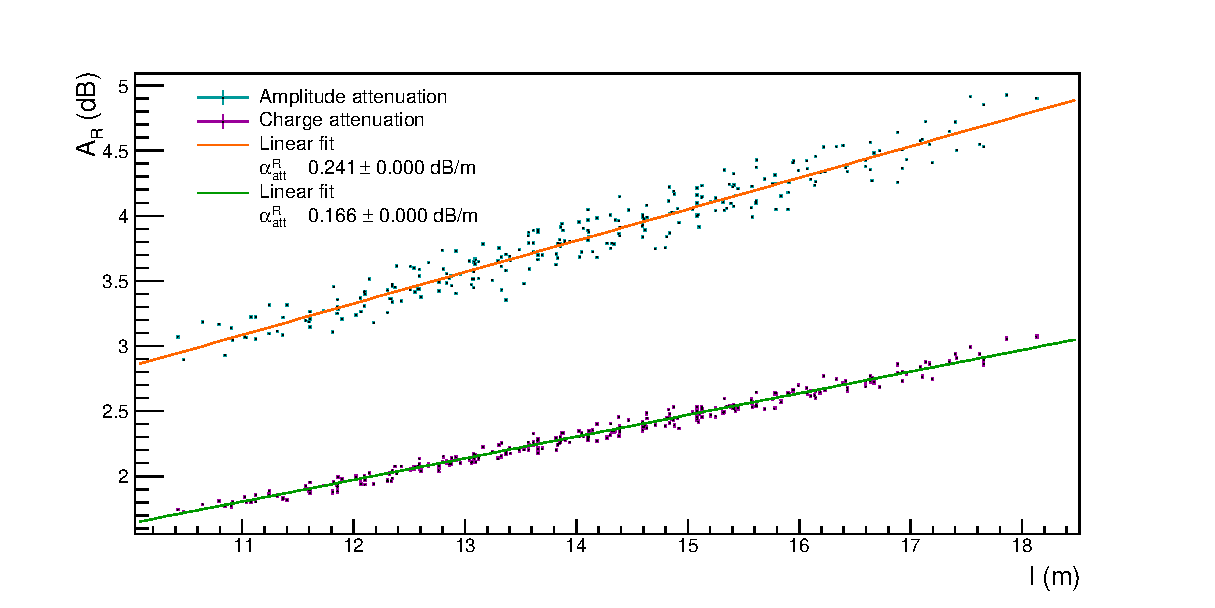
\includegraphics[width=15cm]{commissioning/fig_commissioning/attenuation_length.eps}
  \caption{The amplitude $\mathcal{A}$ is displayed as a function of the measured cable length $l$.
    The data set calculated with the amplitude (charge) is given in cyan (magenta) and fitted by a linear function in orange (green).
    The values of the slope, which represent the linear attenuation of the coaxial cables in dB/m, are respectively $\alpha_{\text{att}}^{\text{R, amp}} = 0.241\pm 0.000$dB/m and $\alpha_{\text{att}}^{\text{R, ch}} = 0.166\pm0.000$dB/m.
    The two $y$-intercept values, which represent the reflection of the pulse on the PMT divider, are $f_{r}^{amp} = 0.402\pm 0.032$ dB and $f_{r}^{ch} = -0.020\pm 0.013$ dB.
    \label{fig:attenuation}}
\end{figure}
The values of $\alpha_{\text{att}}^{\text{R}}$ and $f_{r}$, for both amplitude and charge cases, are displayed in the legend.
Firstly, the two linear fits reveal that, whether calculated with the amplitude, or with the charge, the linear attenuation $\alpha_{\text{att}}^{\text{R}}$ is smaller than the calculated one $\alpha_{\text{att}}^{\text{th}}$ (for the amplitude case, $\alpha_{\text{att}}^{\text{th}}\simeq 5\times \alpha_{\text{att}}^{\text{R, amp}}$, and for the charge case $\alpha_{\text{att}}^{\text{th}}\simeq 7\times \alpha_{\text{att}}^{\text{R, ch}}$).
That means the signal is less affected, when transmitted by the cable, than expected.
Secondly, the attenuation in charge is less important that the attenuation in amplitude.
This can be easily explained: as it is integrated over time, the charge is a quantity less affected by amplitude variations that the amplitude itself.
For the same reason, the charge data set points are less spread than the amplitude ones, meaning that we are less sensitive to cable length variations when using the charge quantity.


This work achieved, we want to verify if no cable was damaged after installation.
Reflectometry also aimed at checking cable conditions by performing waveform shape analysis on secondary pulses.

\subsection{Pulse shape analysis}
\label{subsec:pulse_shape}
In Fig.~\ref{fig:CFD} is displayed an example of \emph{normal} pulse, which corresponds to the case represented in Fig.~\ref{subfig:reflecto_normal}.
In this case, the pulse sent in the cable travels to the PMT, and goes back to the acquisition after reflection on the divider.


\subsection{Comparison with $^{60}$Co}

\subsection{Conclusion}
A faire : regarder le rising time en fonction de la longueur du cable

\section{Calibrating the electronic boards}
\label{sec:TimeSynchroFEB}

\subsection{Principle}
\subsection{Measuring the time offset of front end boards}
\subsection{Results}


\section{Energy calibration of optical modules}
\label{sec:comm_energy_calibration}


*thèse Arnaud page 103*

As described in Sec.~\ref{subsec:OMtimeResponse}, the collected charge at PM voltage divider is proportional to the amount of incident photoelectrons, and then to the initially deposited energy inside the scintillator.
Once optical modules were assembled (optical coupling, packing, shielding integration), they were individually tested at Bordeaux laboratory, CENBG, with an electron spectrometer [ref].
Their energy resolutions for $1$ MeV-electrons at the centre of scintillator front face were determined.
High voltages were set to optimal values, to obtain an amplitude of $300$ mV for $1$ MeV electrons.
However, after calorimeter integration, due to different environment, amplitude spectra of each optical block have to be re-aligned.
This work was performed by Axel Pin, PhD student at CENBG.
We give in this section a summary of this energy calibration study.

*A finir\\




\section{Baseline studies}
\label{sec:comm_baseline}

\section{Light Injection System}
\label{sec:LI}






\chapter{Characterisation of the calorimeter time resolution}

The precise knowledge of the different particle interaction times in the optical modules of the SuperNEMO calorimeter is important to better understand and reject the background.
For example, the study of electron time-of-flight allows us to distinguish internal events (occurring within the source foils) from external events (radioactive decays occurring outside the source foils, for example in the PMTs or in the iron shielding).

During the commissioning phase, a lot of work, presented in Chapter~\ref{ch:commissioning}, was achieved to calibrate the detector.
Following on from this task and completing it, a great part of the present thesis was allocated to determine the time resolution of the SuperNEMO calorimeter, and to provide tools to purchase this analysis.

In this chapter we present different studies conducted in order to characterise the time response of the SuperNEMO optical modules.
Although the goal of the presented studies is to characterise the time resolution of the SuperNEMO calorimeter, some detector adjustments were still ongoing at the time of the acquisition, that could influence the presented results.
Especially, the energy calibration described in Sec.~\ref{sec:comm_energy_calibration} was not complete, and the Light Injection System presented in Sec.~\ref{sec:LIS} was not yet fully operational.
However, all the work presented here is necessary in the framework of the first calorimeter calibration.
Moreover, I provide all the analysis tools for the collaboration, with a view to doing a possible update, once the whole demonstrator construction will be complete.

The first study presented in this chapter focuses on the characterisation of the time resolution of the SuperNEMO calorimeter, using a calibration source made of Cobalt $60$.
In the second part of this chapter, we study the possibility to gather informations on the calorimeter time resolution using the Light Injection System, a set-up initially designed to calibrate in energy the calorimeter.

%%%%%%%%%%%%%%%%%%%%%%%%%%%%%%%%%%%%%%%%%%%%%%%%%%%%%%%%%%%%%%%%%%%%%%%%%%%%%%%%%%%%%%%%%%%%%%%%%%%%%%%%%%%%%%%%%%%%%%%%%%%%%%%%
\section{Interaction of particles in the SuperNEMO scintillators}
\label{sec:scintillator_interactions}

Understanding how particles interact in the SuperNEMO scintillators is essential.
The calorimeter part of the demonstrator mainly aims to detect electrons and photons.
In this section, we review ***.


\subsection{Interaction of electrons}

Electrons interact with matter through one of two processes: elastic scattering on a nucleus, or inelastic scattering from an atomic electron.
Inelastic scatterings are dominant for polystyrene scintillators and occur through two different forms: coherent scattering with the electron cloud, and radiative energy losses (the so-called bremsstrahlung effect).
In Fig.~\ref{subfig:electron_attenuation} is displayed the stopping power of electrons in polystyrene for these two processes.
\begin{figure}[h]
  \centering
  \begin{subfigure}[t]{0.48\textwidth}
    \centering
    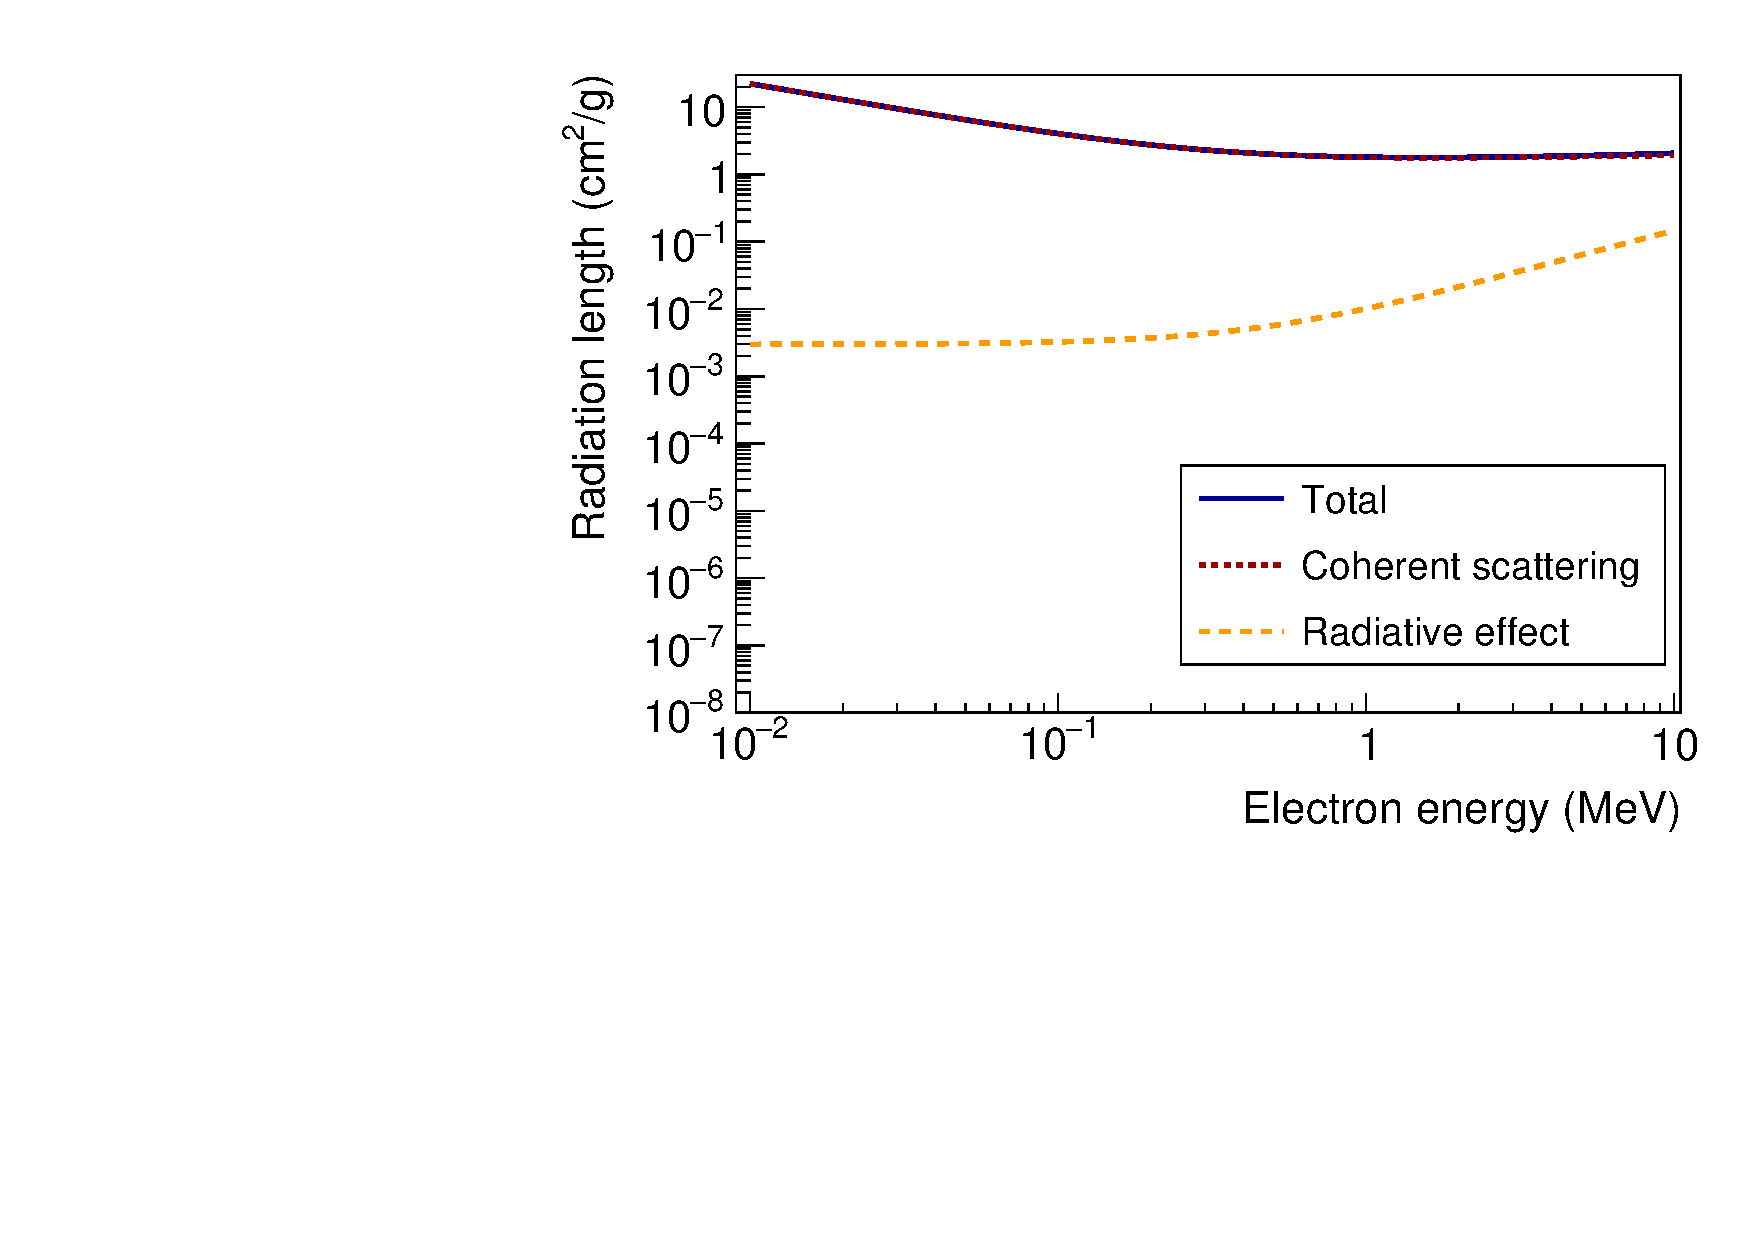
\includegraphics[width=1\textwidth]{commissioning/fig_commissioning/electron_energy_loss.pdf}
    \captionsetup{justification=centering}
    \caption{
      \label{subfig:electron_attenuation}}
  \end{subfigure}
  \hfill
  \begin{subfigure}[t]{0.48\textwidth}
    \centering
    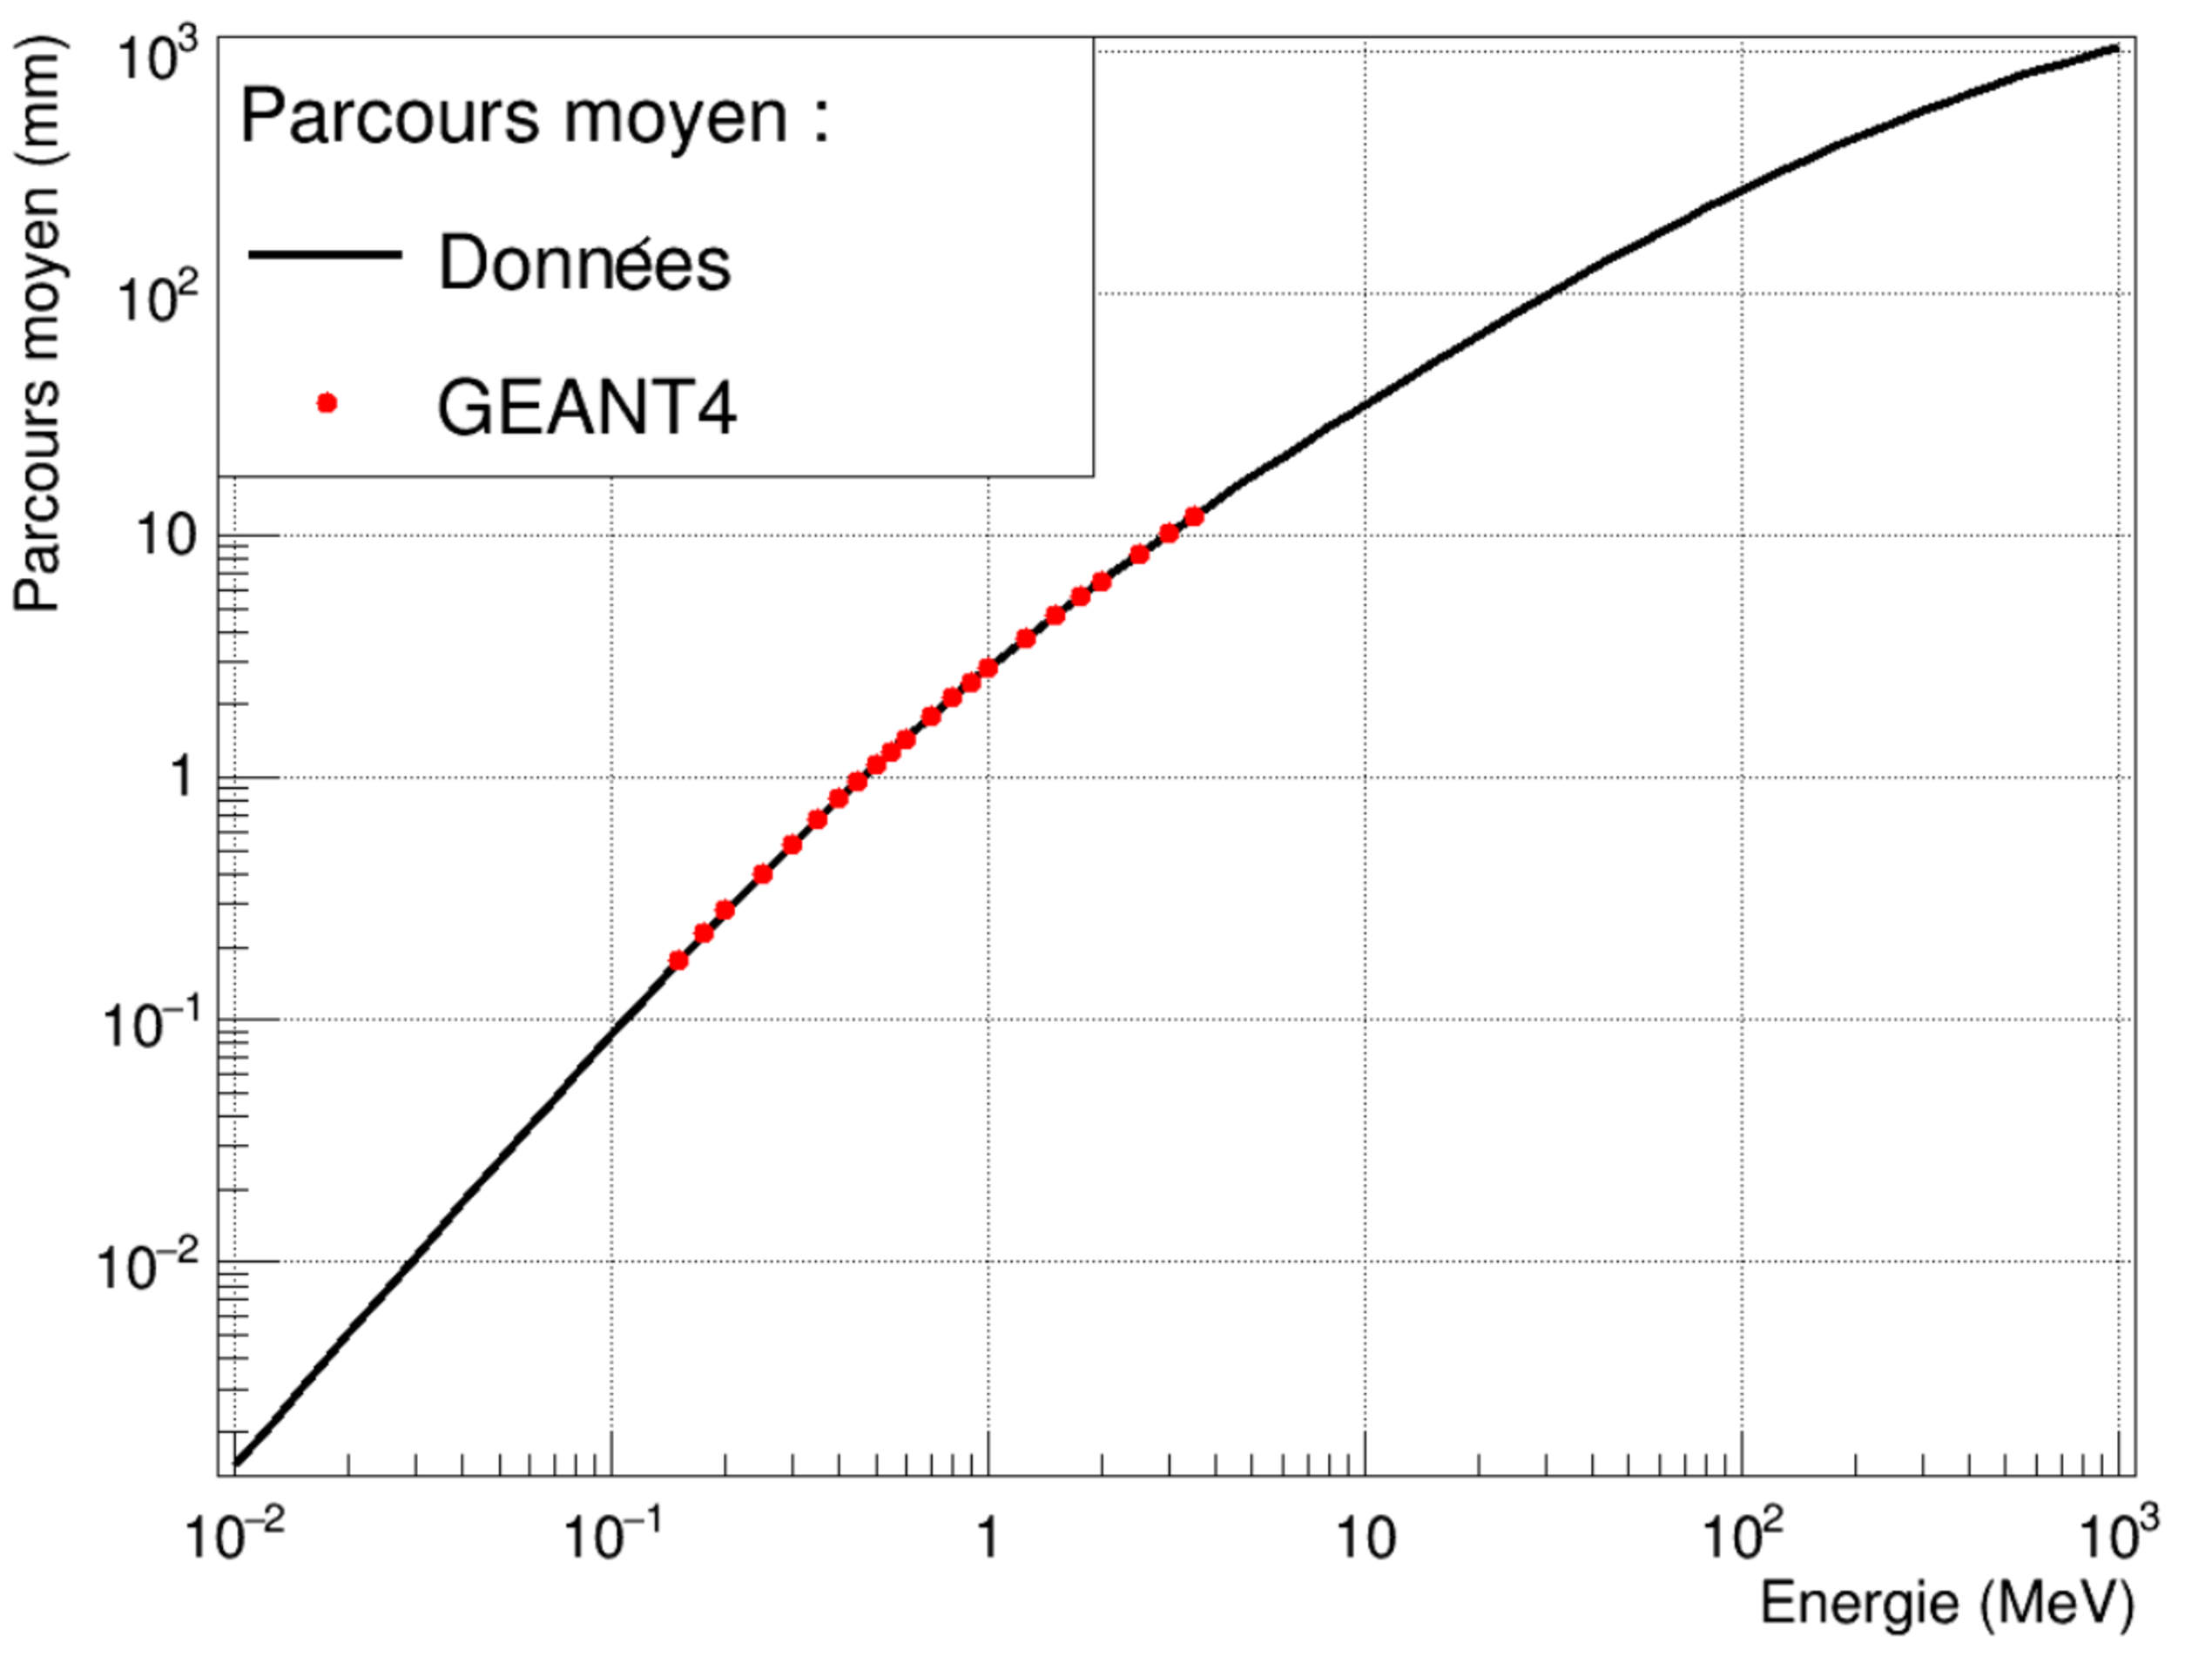
\includegraphics[width=1\textwidth]{commissioning/fig_commissioning/free_path_electrons.pdf}
    \captionsetup{justification=centering}
    \caption{\label{subfig:electron_free_path}}
  \end{subfigure}
  \caption{Stopping power (a) and mean free path (b) for electrons in polystyrene.
    (a) Energy losses through radiative effect (orange dashed line) and coherent scattering (red dashed line), which is the dominant process for the considered energy range.
    %  operate mainly through coherent scattering.
    (b) At $1$ MeV, the mean free path of an electron is about $3$ mm.
  }
\end{figure}
Electrons detected in the SuperNEMO calorimeter should deposit a minimal energy of $50$ keV (the acquisition low energy threshold) and a maximal energy of few MeV (depending on the $\twonu$ isotope).
In this energy range, collisions with the electron cloud are preponderant compared with radiative energy losses.
In Fig.~\ref{subfig:electron_free_path}, we give informations about the mean free path of an electron in polystyrene.
In particular, we observe that an electron of $1$ MeV penetrates, in average, several millimetres into a polystyrene scintillator.


\subsection{Interaction of photons}

Photons travelling in  matter can interact with the electronic cloud, through $3$ main processes, whose contributions are presented in fig.~\ref{subfig:photon_energy_loss}, depending on their energies.
\begin{figure}[h]
  \centering
  \begin{subfigure}[t]{0.48\textwidth}
    \centering
    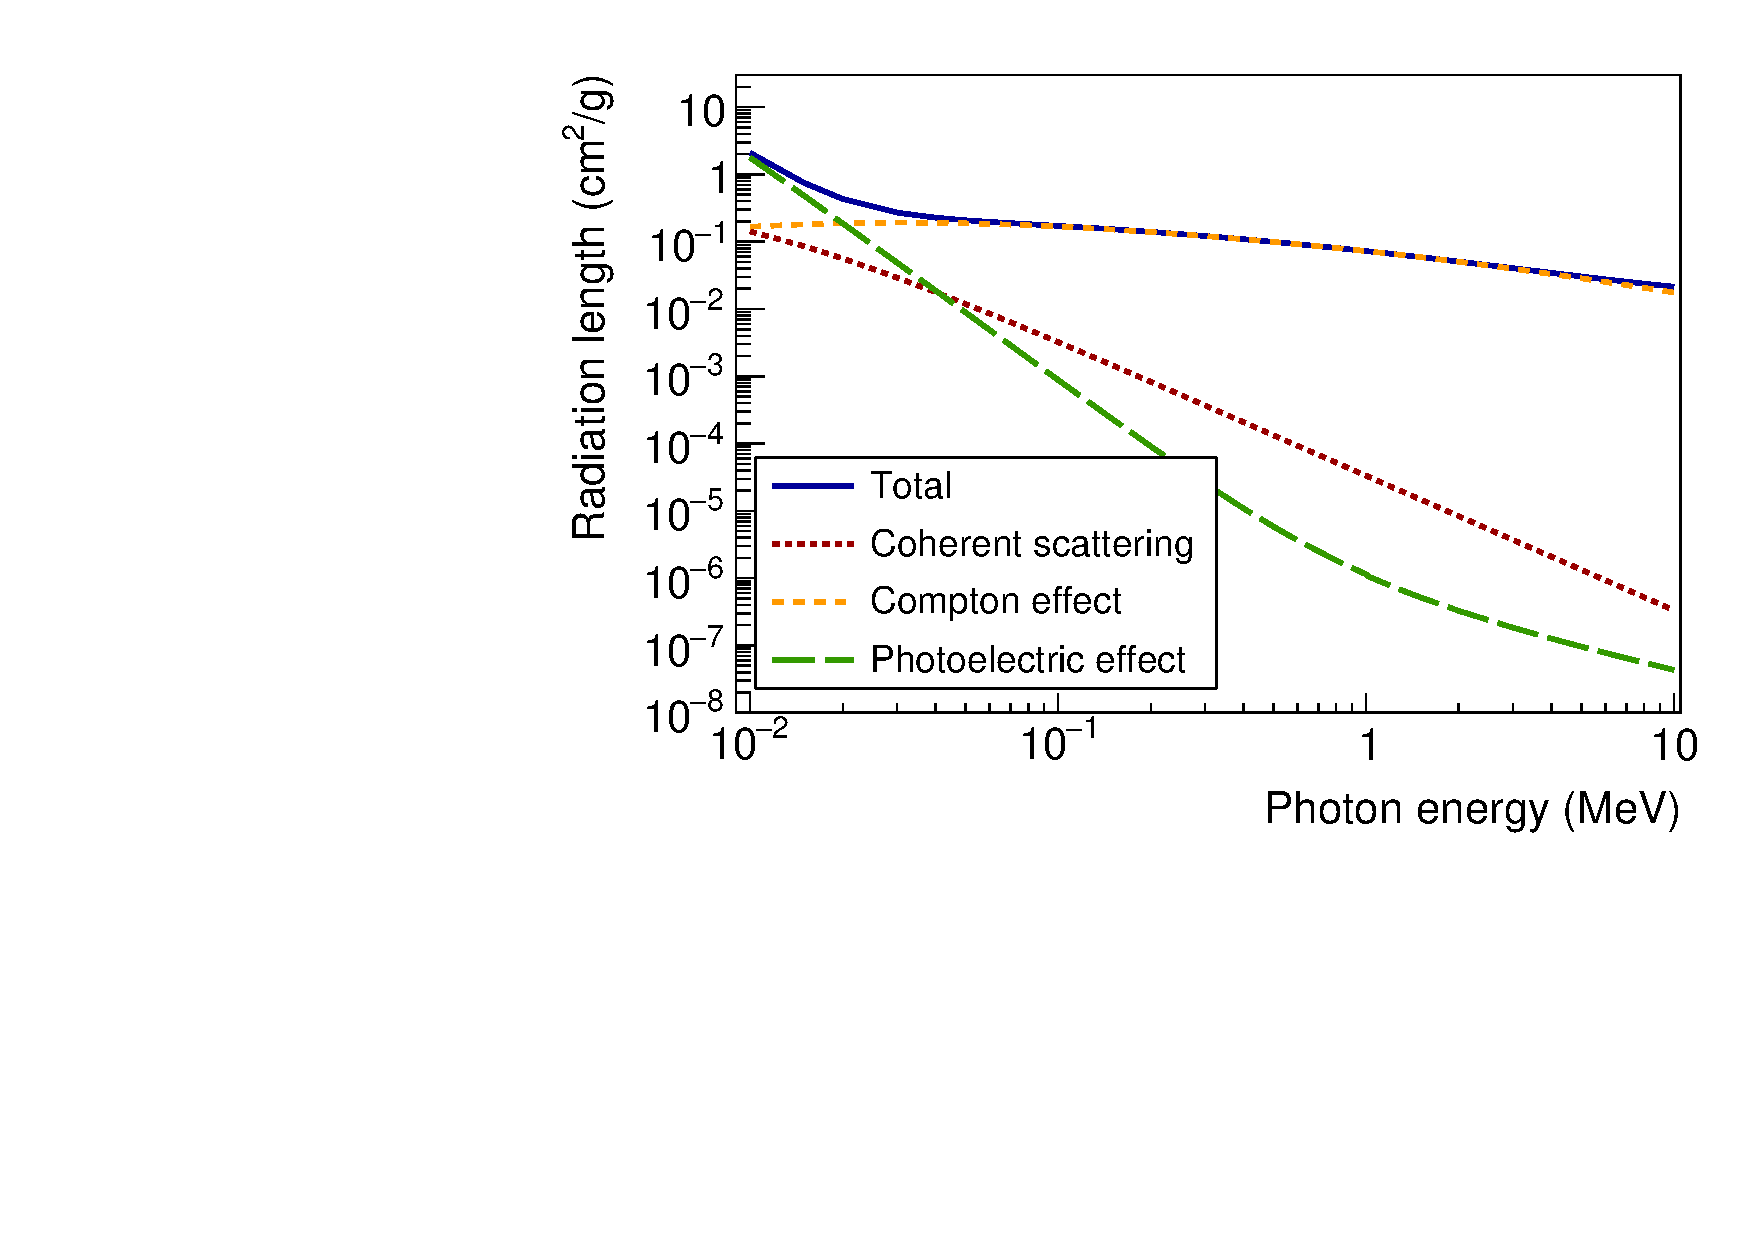
\includegraphics[width=1\textwidth]{commissioning/fig_commissioning/photon_energy_loss.pdf}
    \captionsetup{justification=centering}
    \caption{\label{subfig:photon_energy_loss}}
  \end{subfigure}
  \hfill
  \begin{subfigure}[t]{0.48\textwidth}
    \centering
    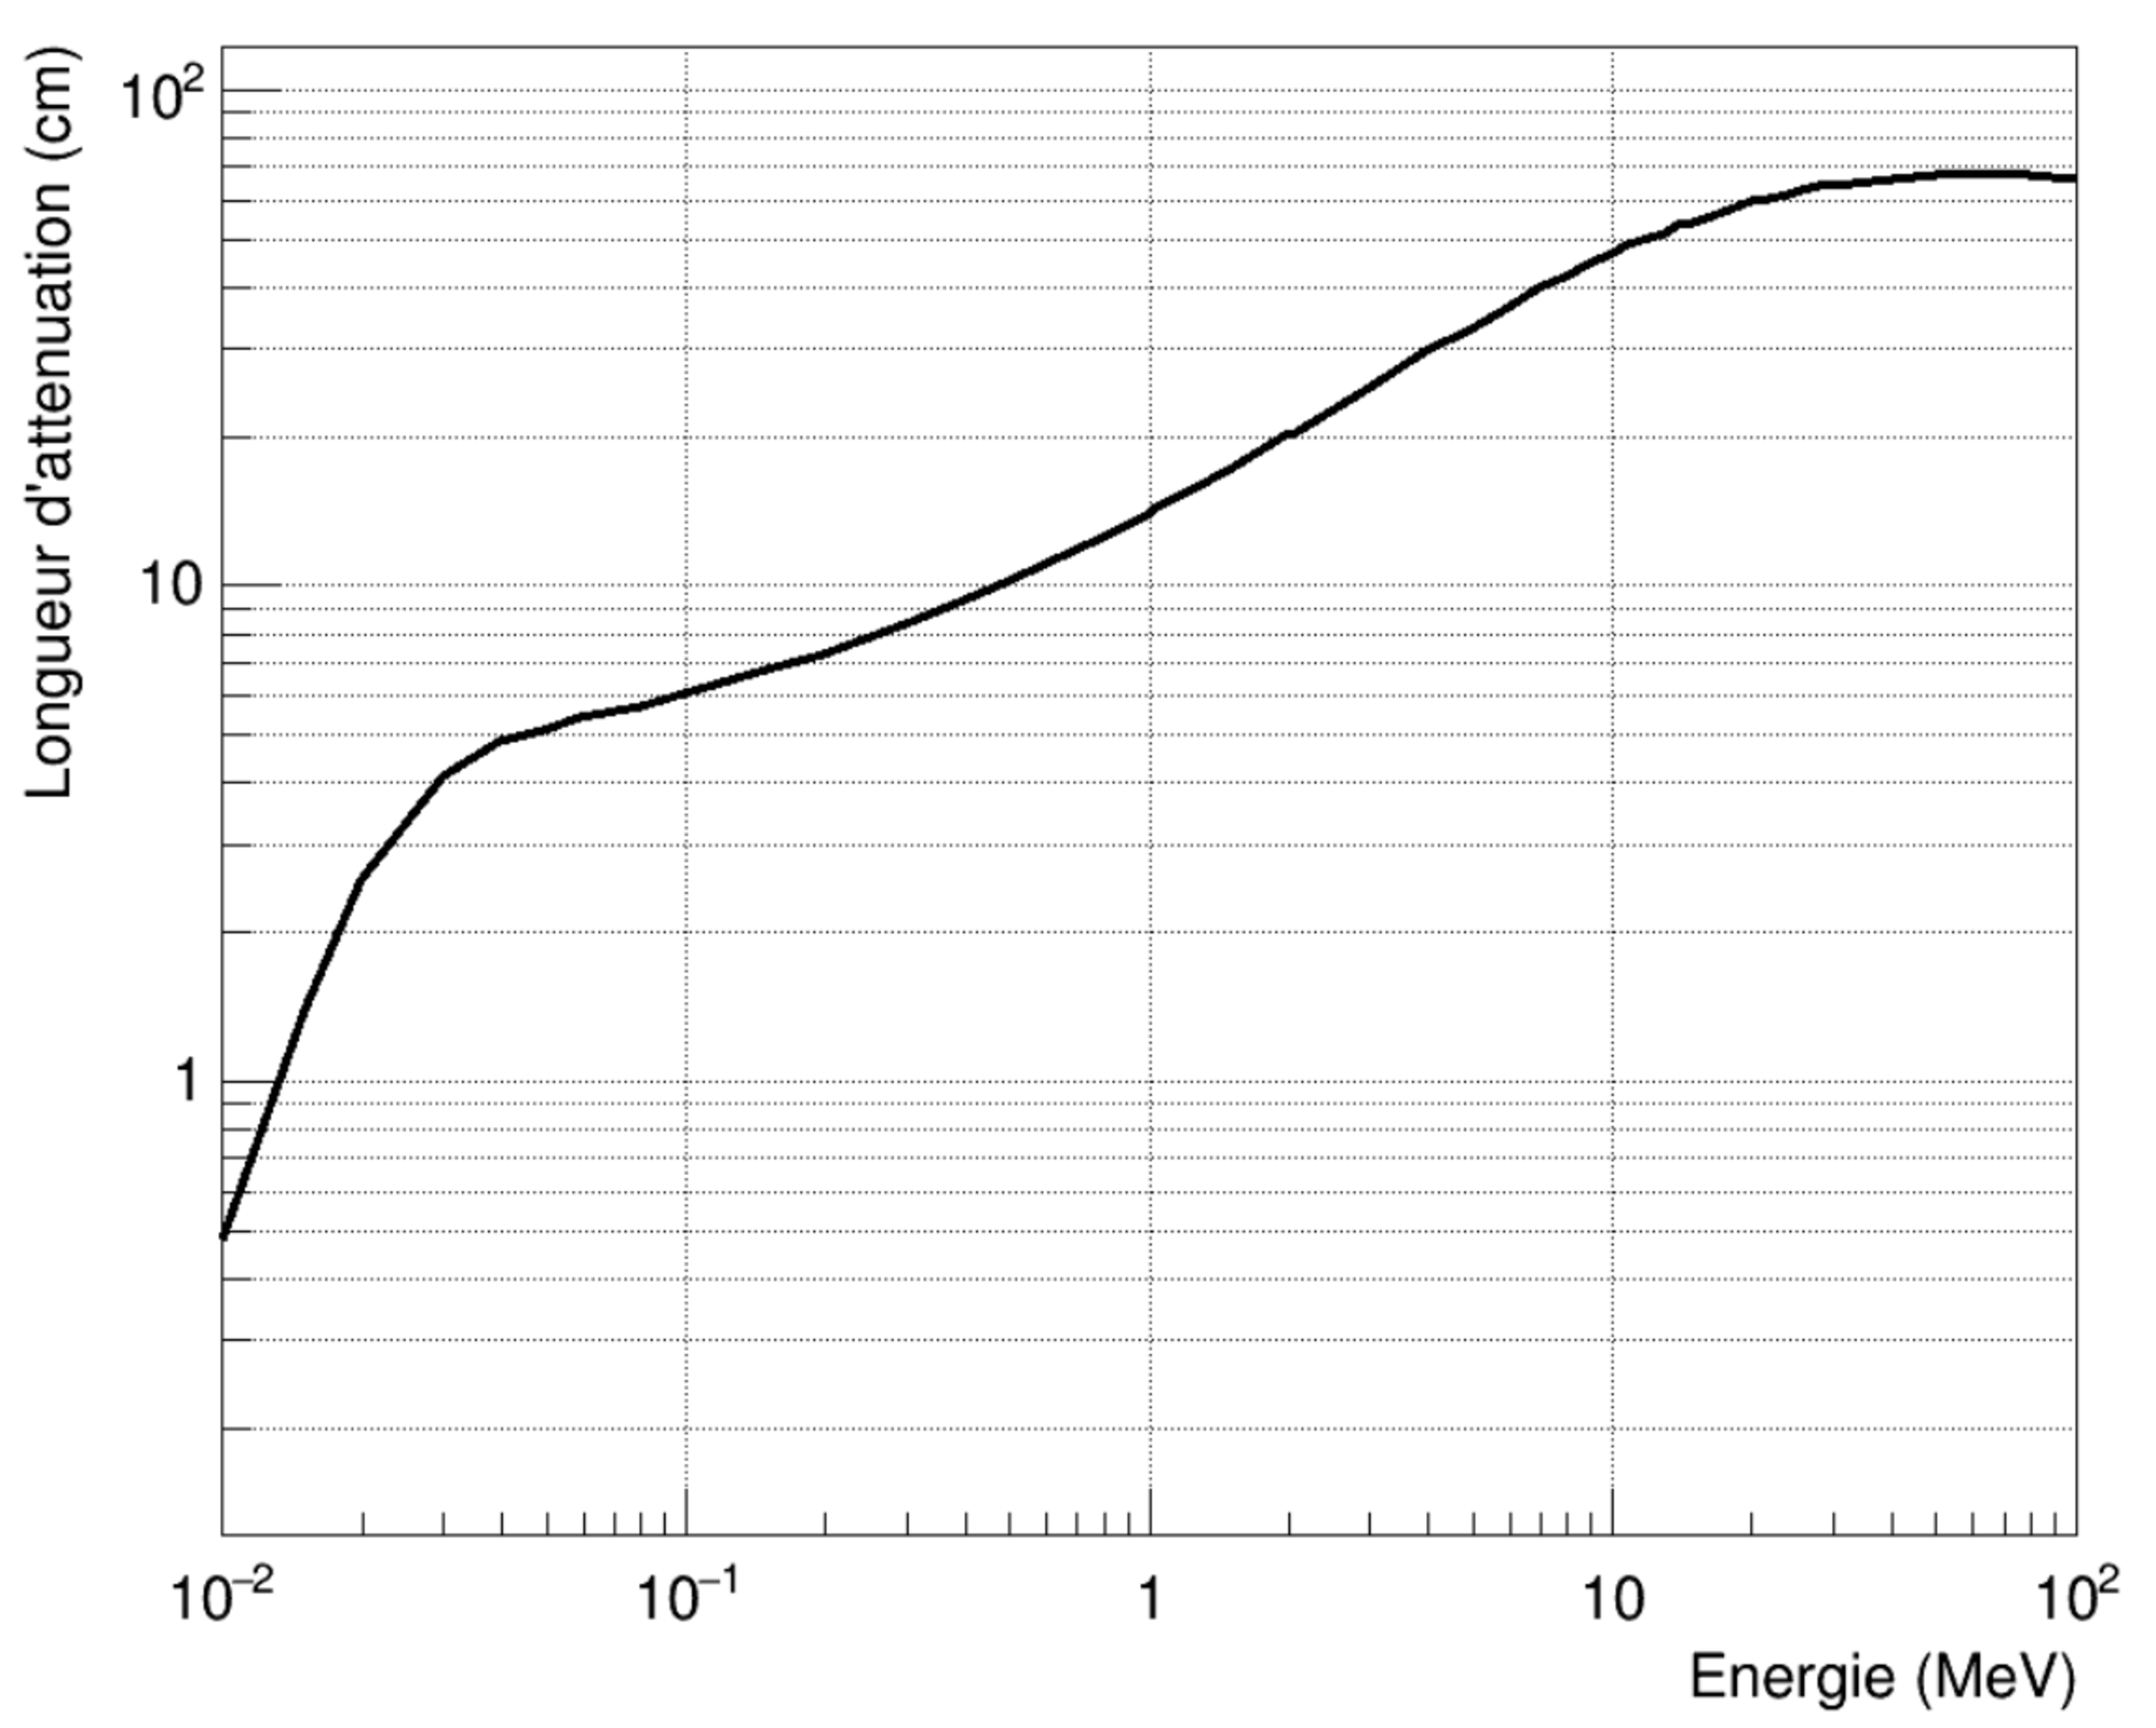
\includegraphics[width=1\textwidth]{commissioning/fig_commissioning/attenuation_length_photons.pdf}
    \captionsetup{justification=centering}
    \caption{\label{subfig:attenuation_length_photons}}
  \end{subfigure}
  \caption{Linear attenuation coefficient (a) and attenuation length (b) for $\gamma$ radiations in a plastic scintillator made of polystyrene.
    (a) In the considered energy range of $10$ keV $ -\; 10$ MeV, $\gamma$ radiations interact with matter mainly through Compton diffusion.
    (b) The attenuation length of a $\gamma$ radiation is about $10$ cm at $1$ MeV.
  }
\end{figure}
Low-energy photons mainly interact with the electron cloud, either through photoelectric effect ($\gamma$ radiation is fully absorbed by an electron of the cloud), or through coherent (so-called Rayleigh) scattering.
But the dominant effect, for energies between $10$ keV and $10$ MeV, is the Compton inelastic scattering of a $\gamma$ with an atomic electron.
In Fig.~\ref{subfig:attenuation_length_photons}, we display the mean attenuation length of a $\gamma$ radiation in polystyrene scintillators, with energy.
Thus, most of $1$ MeV $\gamma$ radiations will interact around $10$ cm inside the scintillating material.\\

At the considered energy range ($10$ keV $ -\; 10$ MeV), the interaction of photons with matter is dominated by Compton effect, while the electrons interact mainly through coherent scattering.
The SuperNEMO scintillators are designed to detect such particles.
Photons have a high probability to interact inside the volume of the scintillator, while electrons are stopped in the first few millimetres.

The following two sections are devoted to the study of the time resolution of the SuperNEMO optical modules.



%%%%%%%%%%%%%%%%%%%%%%%%%%%%%%%%%%%%%%%%%%%%%%%%%%%%%%%%%%%%%%%%%%%%%%%%%%%%%%%%%%%%%%%%%%%%%%%%%%%%%%%%%%%%%%%%%%%%%%%%%%%%%%%%
\section{Measurement of the time resolution with a $^{60}$Co source}
\label{sec:Co_analysis}
This section is dedicated to detail the time resolution study performed using a Cobalt $60$ source, exploiting the time characteristic of two photons emitted during the radioactive disintegration process of this nucleus.
A great proportion of the whole SuperNEMO demonstrator was successfully characterised using this radioactive source.

\subsection{Description of Cobalt $60$ nucleus}
\label{subsec:CoSource}
The Cobalt $60$ is a man-made isotope, with a $5.27$ years half-life, of which we provide the main interesting properties in the simplified decay scheme of Fig.~\ref{fig:Co_decay_scheme}.
\begin{figure}[h]
  \centering
  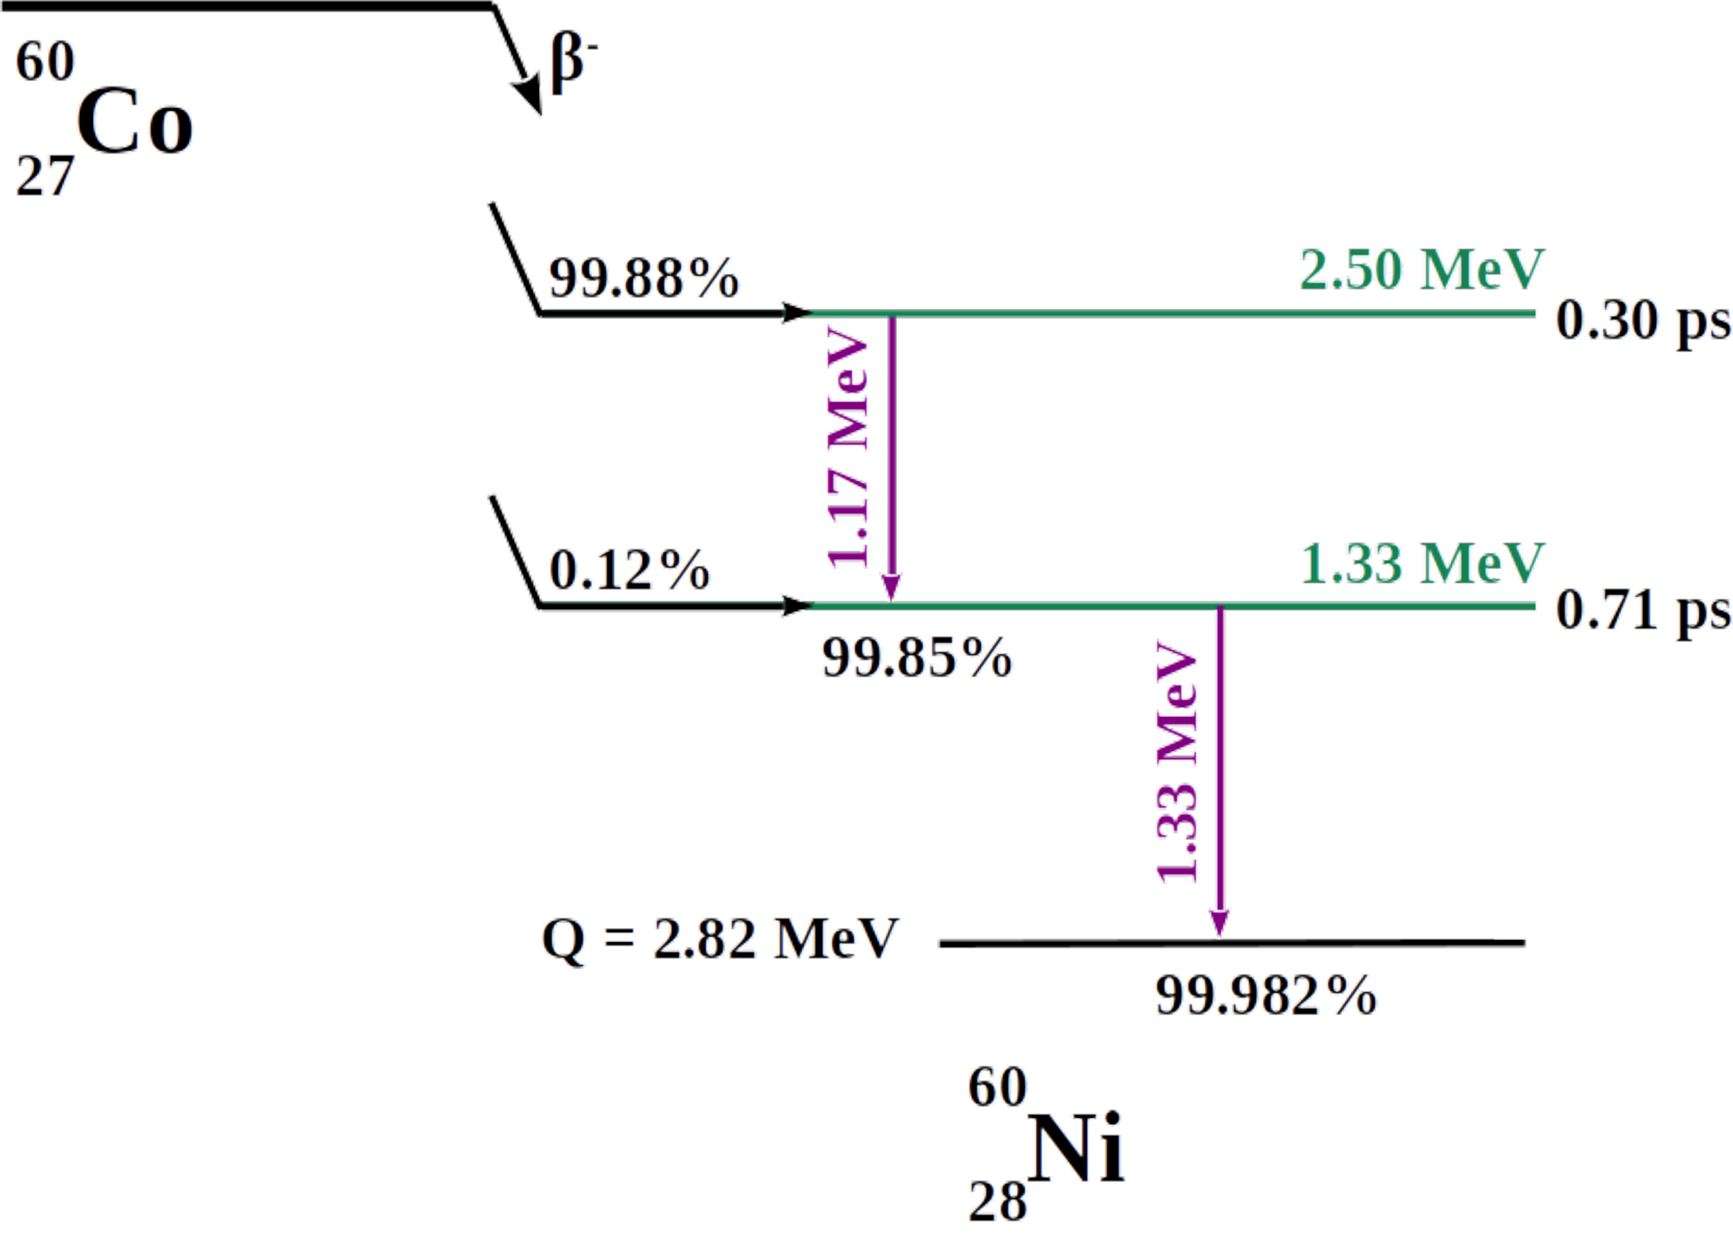
\includegraphics[width=9cm]{commissioning/fig_commissioning/Co_decay_scheme.pdf}
  \caption{A simplified decay scheme for Cobalt $60$ \cite{web:nucleide}.
    The Cobalt decays, through $\beta^{-}$, predominantly to the $2.50$ MeV state.
    Then, two $\gamma$'s (whose energy levels are represented in green) are emitted in $99.83$\% of the cases.
    The two photons have an energy of $1.17$ MeV and $1.33$ MeV, respectively.
    As the life-time of the $1.33$ MeV energy level is short ($<1$ ps) with respect to the timing precision of the calorimeter, the two photons can be considered as emitted in coincidence.
    We use this property to calibrate in time the demonstrator optical modules.
    \label{fig:Co_decay_scheme}}
\end{figure}
This unstable nucleus spontaneously decays, through the $\beta^{-}$ process, into an excited state of Nickel $60$.
To reach the ground state of the Nickel $60$, the nucleus goes through two successive energy levels, emitting two photons of $1.17$ MeV and $1.33$ MeV, respectively.
The life-time of the second energy level is under the picosecond, thus very short with respect to the expected timing precision of the calorimeter.
Therefore, the two photons are considered as emitted in coincidence.

We aim to exploit these two photons emitted after the $\beta^{-}$ disintegration to determine the calorimeter time resolution.

\subsection{Time response of optical modules}
\label{subsec:OMtimeResponse}

In order to characterise incoming charged particles (alphas, electrons), each calorimeter block of SuperNEMO is composed of a scintillator and a photomultiplier.
The purpose of the scintillator material is to stop the incoming particles, which will induce the production of the so-called optical photons.
The optical photons reaching the photomultiplier photocathode are then converted into electrons, with an efficiency called quantum efficiency.
After amplification, electrons are collected by the anode which delivers an electric signal whose charge is proportional to the initial amount of incident photoelectrons.
This signal is then transmitted, via the PM voltage divider, to the electronic readout, where the signal is sampled.
The particle energy, as well as the time of arrival introduced in Sec.~\ref{subsec:timing}, can be extracted from the signal waveform analysis.
Each step of the charged particle detection process, from the incident particle interaction inside the scintillator, to the signal sampling at the electronic readout, can have an impact on the precise time measurement of the charged particle.
We introduce the so-called calorimeter time resolution $\sigma_t$, which encapsulates the global uncertainty on the time-arrival measurement of particles into the calorimeter.
The squared time-resolution can therefore be expressed as the sum of two contributions:
the scintillator resolution $\sigma_{t, \textrm{sc}}^{2}$, and the PMT resolution $\sigma_{t, \textrm{PM}}^{2}$,
\begin{equation}
  \sigma_{t}^{2}=\sigma_{t,\text{sc}}^{2}+\sigma_{t,\text{PM}}^{2}\,.
  \label{eq:Co_sigma_t}
\end{equation}
In the following, we detail in depth the physical origins of these terms.

\subsubsection*{Scintillator time dispersion}
The scintillator temporal dispersion $\sigma_{t,\text{sc}}$ in Eq.~\eqref{eq:Co_sigma_t} receives contributions mainly from two important characteristics of the scintillator operating principle.

\paragraph{Interaction point:}
The incoming particle's interaction point location inside the scintillator block highly contributes to the scintillator temporal uncertainty, and depends on the incident particle type.
In fact, this effect will not have the same impact on time dispersion, depending on whether the incident particle is a photon or an electron.
In Fig~\ref{fig:photon_scintilator} are schemed the interactions of a photon and that of an electron for the specific case of a SuperNEMO plastic scintillator.
\begin{figure}[h]
  \centering
  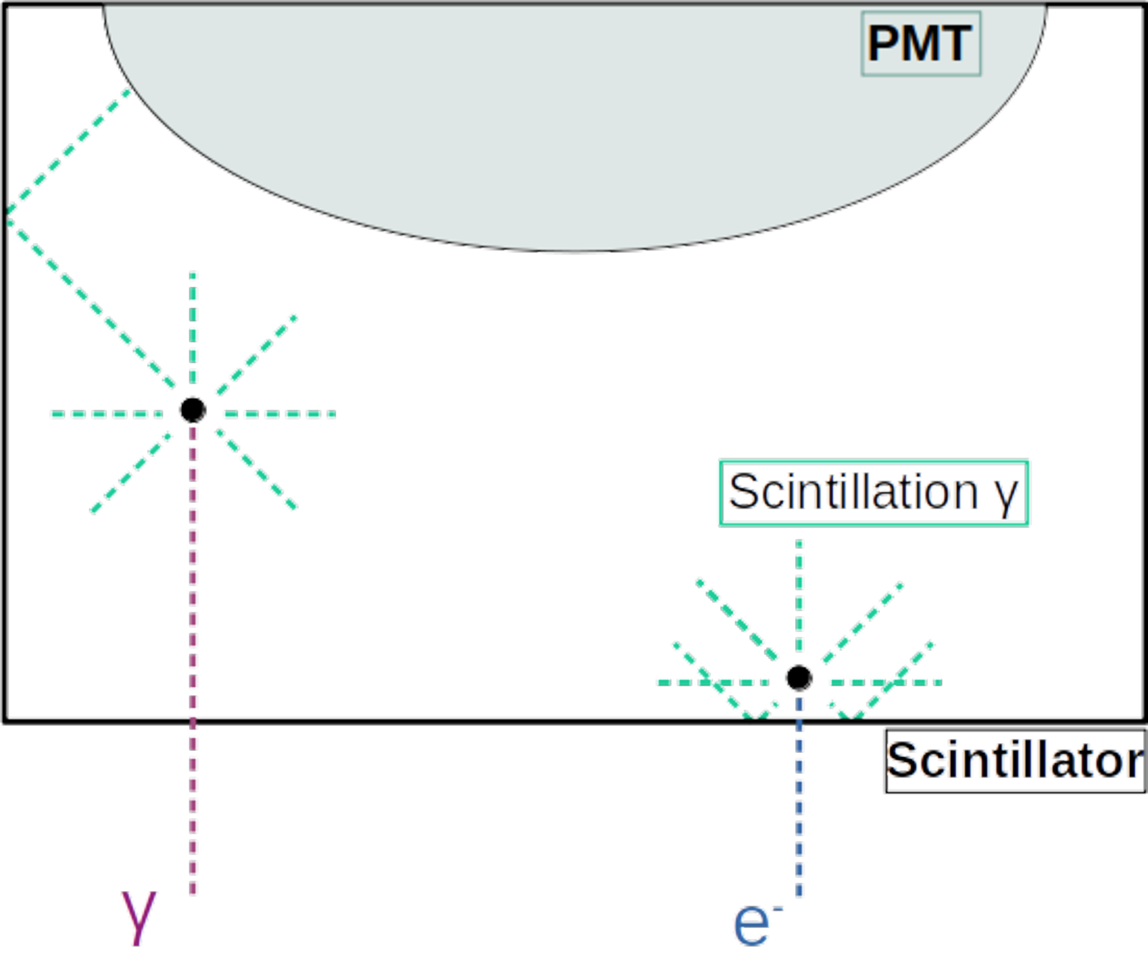
\includegraphics[width=8cm]{commissioning/fig_commissioning/Co_multi_reflection.pdf}
  \caption{A scheme of interaction of particles in a scintillator.
    The photon case is displayed on the left in pink dotted line, and the electron case is on the right in dark blue dotted line.
    Both particles enter in the scintillator through the front face.
    Examples of interaction points inside the scintillator are represented by the black dots.
    The photons of scintillation emitted isotropically after the interaction are materialised by the bright green dotted lines.
    Due to different interaction probabilities in matter, the two particles intercat at different depths inside the scintillator.
    The photon can interact deeply inside the volume, while the electron has a high probability to stop within the first few millimetres.
    \label{fig:photon_scintilator}}
\end{figure}
In Sec.~\ref{sec:scintillator_interactions}, we exposed the different interaction types of photons and electrons.
We have also explained the origin of the differences that exist in terms of interaction depth between these two types of particles.
To remain consistent with these conclusions, we represent the electron as interacting in the first millimetres, while the photon stops deep inside the scintillator.
When a particle (photon or electron) interacts in the scintillating material, the absorbed energy leads to the isotropic emission of scintillation photons:
they propagate inside the scintillator, in all directions from the interaction point, at the speed of $c/n_{sc}$, with $n_{sc}$ the optical index of polystyrene, and $c$ the light speed in vacuum.
Depending on their initial direction, some of those photons propagate straight to the PMT (we name them the \emph{direct} photons), while others are at least reflected once on the scintillator surface, before reaching the PM glass.
This mechanism leads to time delays between direct and reflected photons.

In order to illustrate, and give an order of magnitude of this delay, let us consider an example where an incoming $\gamma$ particle enters a scintillator from the front face, and interacts right in the centre of the scintillator volume.
After the scintillation emission process, a direct photon will reach the PM glass surface at time
\begin{equation}
  t_{s} = \frac{L}{2c/n_{sc}}\,,
\end{equation}
$L$ being the scintillator width.
Now, let us consider another photon, that we name \emph{backward reflected}, emitted in the opposite direction.
It will propagate, reflect on the front scintillator surface, and finally reach the PM at
\begin{equation}
  t_{r} = \frac{3L}{2c/n_{sc}}\,.
\end{equation}
This reflected photon is therefore delayed compared to the direct photon, with a time-shift of
\begin{equation}
  \Delta t^{r,s} = t_{r} - t_{s} = \frac{L}{c/n_{sc}}\,.
\end{equation}
In the case of a SuperNEMO scintillator, the length $L$ has been designed to $25$ cm, and the optical index is the one of polystyrene with $n_{sc}=1.5$.
Finally, for an incoming particle interacting at the centre of a SuperNEMO scintillator volume, a backward reflected scintillation photon will reach the PM glass $1.25$ ns later than a direct photon.
And this delay is even more important as the incident particle interacts deep inside the scintillator.

In view of the conclusions given in Sec.~\ref{sec:scintillator_interactions}, we know that photons have a higher probability of interacting far into the scintillator block, compared with electrons.
Therefore, this time-shift effect is all the more important for incoming photons, while it is quite negligible for incoming electrons, for which reflected photoelectrons reach the PM glass almost as the same time as the direct ones.

This mechanism increases the signal collection rising time at the PM anode, and boosts the scintillator time dispersion $\sigma_{t,\text{sc}}$, with $\sigma_{t,\text{sc}}^{\gamma}>\sigma_{t,\text{sc}}^{\text{e}^{-}}$.

\paragraph{Scintillating light emission:}
When a particle interacts in a SuperNEMO scintillator, two successive mechanisms of light absorption/re-emission take place.
Firstly, the excitation of scintillator molecules leads to the creation of fluorescence photons.
Afterwards, those optical photons are absorbed, then re-emitted by the POPOP agent, at higher wavelengths (for more details, we refer to Sec.~\ref{subsec:SN_calo} of Chapter~\ref{ch:detector}).
The characteristic times of these two processes contribute to increase the scintillator time dispersion $\sigma_{t,\text{sc}}$.\\
%% These two processes follow the same temporal distribution
%% \begin{equation}
%%   \mathcal{N}_{\text{photons}} = A\times e^{-t/\tau}\,,
%%   \label{eq:fluorescence_photons_time}
%% \end{equation}
%% with $\mathcal{N}_{\text{photons}}$ the number of generated photons at time $t$, $A$ a normalisation constant and $\tau$ the fluorescence characteristic time of the considered process.

Now that two main contributions accounting for the uncertainty on time measurement taken by the scintillator had been developed, we detail the origin of the second term of Eq.~\eqref{eq:Co_sigma_t}, $\sigma_{t,\text{PM}}$.

\subsubsection*{Photomultiplier time dispersion}

A photomultiplier is a photodetector: after the light is collected and converted at the photocathode, the photoelectrons are multiplied.
The transit time for the photoelectrons emitted at the photocathode to reach the anode after being multiplied is not constant for every photoelectron, due to a varying path for electrons emitted by the different dynodes.
This results in a timing dispersion.
This fluctuation is called transit time spread (TTS).
It leads to an uncertainty on the time measurement and so has an influence on the photomultiplier time dispersion $\sigma_{t,\text{PM}}$.\\

In the following, we describe how we characterised the time dispersion brought by the optical module on the time measurement, using a Cobalt 60 source.


\subsection{Final experimental design}
\label{subsec:Co_setup}


The idea to use a Cobalt $60$ source to characterise the time response of the calorimeter part of SuperNEMO had never been tested before the current analysis.
Therefore, all the experimental design had to be implemented.


\subsubsection*{Setting up the experimental design}


The initial activity of the Cobalt source we used for this experimental set-up was $447.4$ kBq in February $2014$.
Given the half-life of this isotope, it was reduced to $232$ kBq at the time of the data-taking.
In order to determine the best design, and later to monitor and compare the results obtained in the framework of this analysis, I performed simulations of \Co\ disintegrations with the source activity at the time of the data-taking, for the demonstrator configuration.
The characteristics of those simulations are detailed later in this section.

As the demonstrator was closed at this time, it was impossible to set the Cobalt source inside the detector, at the source foils level.
Hence, the calibration source was placed behind the calorimeter, as displayed in Fig.~\ref{subfig:Co_setup}, where we can distinguish a side view of the calorimeter.
\begin{figure}[h]
  \centering
  \begin{subfigure}[t]{0.48\textwidth}
    \centering
    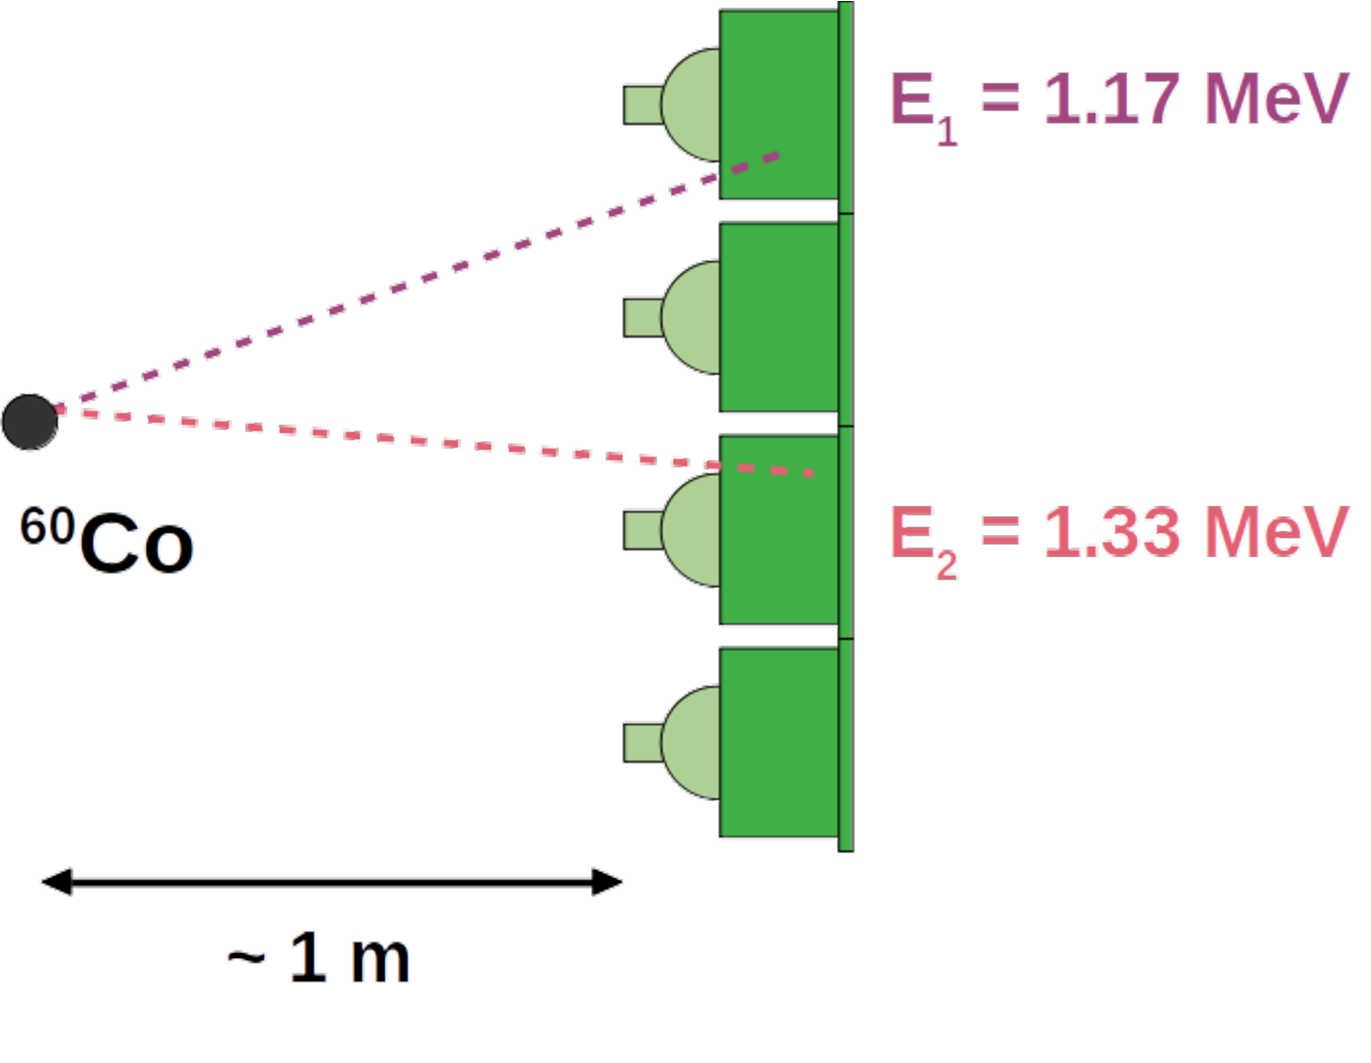
\includegraphics[height=0.5\textwidth]{commissioning/fig_commissioning/Co_setup.pdf}
    \captionsetup{justification=justified}
    \caption{
      \label{subfig:Co_setup}}
  \end{subfigure}
  \hfill
  \begin{subfigure}[t]{0.48\textwidth}
    \centering
    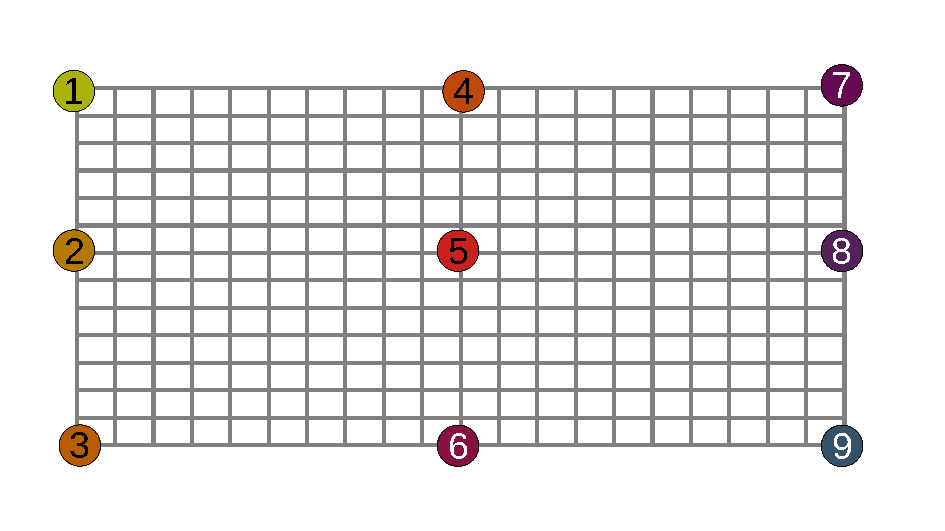
\includegraphics[height=0.5\textwidth]{commissioning/fig_commissioning/Co_setup_wall.pdf}
    \captionsetup{justification=justified}
    \caption{
      \label{subfig:Co_setup_wall}}
  \end{subfigure}
  \caption{(a) Side view example of the Cobalt source positioning behind a calorimeter main wall, schemed by $4$ optical modules (green).
    The emissions of the $2$ $\gamma$'s of interest are displayed in coloured dotted lines.
    (b) Front view of the nine source positions behind a main wall.
    Each grey box represents an optical module.
  }
\end{figure}

As described in Chapter~\ref{ch:detector}, the SuperNEMO calorimeter is composed of two main walls (called \emph{French} and \emph{Italian} sides), as well as the so-called X-Walls (on the detector sides) and $\gamma$-Vetos (on top and below the detector).
At the time of the data-taking, X-Walls and $\gamma$-Vetos were not yet operational, hence the current analysis only applies on the French and Italian main calorimeter walls.
In order for all PMs to detect $\gamma$'s from Cobalt decays, several bunches of data acquisitions were taken:
the source was placed at $9$ different positions on each of the $2$ main calorimeter walls, approximately one meter behind.
Therefore, in total, $19$ data acquisitions have been taken, of which:
\begin{itemize}
\item $18$ with the Cobalt source set behind the wall. The $9$ different positions for one wall are represented in Fig.~\ref{subfig:Co_setup_wall}.
\item $1$ acquisition have been taken without the Cobalt source, with the Italian main wall, to characterise the background detected with the current calorimeter settings.
\end{itemize}
Each data acquisition lasted about $25$ minutes, for a total of $10$ hours of on-site activities, taking into account the time needed to move the Cobalt source from spot to spot.

Currently, the demonstrator is not protected from the laboratory lights by the anti-radon tent.
As laboratory lights would damage the SuperNEMO photomultipliers, two removable black curtains are deployed on top of the detector, and acquisitions are taken in dark laboratory.
With this way of doing, data acquisitions can be performed, while eventual necessary repairs remain possible during the detector commissioning.
Nevertheless, taking acquisitions in the dark is a big constraint.
Moreover, the source, initially used for teaching purposes, was loan by IPN laboratory (Orsay), for only two weeks, mainly because of legal constraints.
Therefore, to not disturb LSM on-site activities (and to make the loan time profitable), a SuperNEMO team and I performed night shifts to take data.
The acquisition took place during two weeks, at the summer break $2019$.

\subsubsection*{Simulated data}

*sigma t !!*

\paragraph{Cobalt events simulations:}
As for the data acquisition, the simulated source has been placed behind the calorimeter walls.
Hopefully, there was no need to simulate all the $18$ positions.
In fact, at this time, the detector implemented in simulations is symmetrical in terms of detection performances.
Therefore, simulations of \Co\ events behind the two main walls are equivalent, and we only need to simulate events from $4$ locations (positions $1$, $2$, $4$ and $5$, according to the Fig.~\ref{subfig:Co_setup_wall} numbering system), other being obtained by symmetry operations.
I used the Falaise software to perform these simulations.
Four data-taking, for a total of $10^{9}$ Cobalt events, were simulated, using the IN$2$P$3$ computing centre platform.
A visualisation, provided by the Falaise Software, of a simulated Cobalt event behind the Italian calorimeter main wall, is shown in Fig.~\ref{fig:Co_visu}.
\begin{figure}[h]
  \centering
  
\includegraphics[width=6cm]{commissioning/fig_commissioning/Co_visu.pdf}
  \caption{Visualisation of a simulated Cobalt event.
    \label{fig:Co_visu}}
\end{figure}
All the simulations carried out as part of this study have been made available to the collaboration.

\paragraph{Background events simulations:}
Currently, the Falaise software does not supply a complete set of background events simulations for the demonstrator design.
This will be implemented as soon as the final demonstrator performances has been determined.
Thus, we did not have at our disposal background events simulations for this analysis.\\

The entire experimental set-up was designed and carried out by me and a group of physicists from LAL, Orsay and LPC, Caen.
I developed a complete set of ROOT codes for data processing and analysis, available on the GitHub platform\footnote{Link to my GitHub page: \href{https://github.com/girardcarillo}{https://github.com/girardcarillo}}.

\subsection{Signal events selection}
\label{subsec:Co_datacut}

We aim to use the two $\gamma$'s of $1.17$ MeV and $1.33$ MeV from Cobalt $60$ $\beta^{-}$ decay, to characterise the time resolutions of individual optical modules.
Thus, the signal we are looking for is two particles detected in coincidence in distinct optical modules.
In order to maximise the signal to background ratio, some selections have been applied on data.
\begin{itemize}
\item Trigger criteria:\\ as we look for two calorimeter hits, we only keep events with exactly two triggering electronic channels.
  Moreover, we are interested in events with two hits which passed both the high amplitude threshold, corresponding to approximately $150$ keV.
  *est-ce que c'est vraiment utile ? pcq on a le cut à 0.7 MeV donc bon ...*
\item Coincidence time criterion:\\ we define the coincidence time-window by events occurring in a $62.5$ ns-long time interval.
  This allows to avoid accidental coincidence events (interactions of two gammas, produced by different sources, in two optical modules), while keeping events where two $\gamma$ particles interact at both ends of the wall.
  This time-window was set for the data-taking and can be improved for eventual future acquisitions.
\item Individual energy selection:\\ given the two photon energies, we only select individual calorimeter hit energies greater than $0.7$ MeV, to reject double Compton interactions of one single photon from Cobalt in different optical modules.
  This energy selection is sufficient for \Co\ $\gamma$ particles, but not for background such as \Tl.
  Moreover, it highly depends on the calibration discussed in Sec.~\ref{sec:comm_energy_calibration}.
  We show in Fig.~\ref{fig:Co_energy_cut} the highest energy hit with the lowest one, for simulated data with \Co\ source in position $5$.
  \begin{figure}[h]
    \centering
    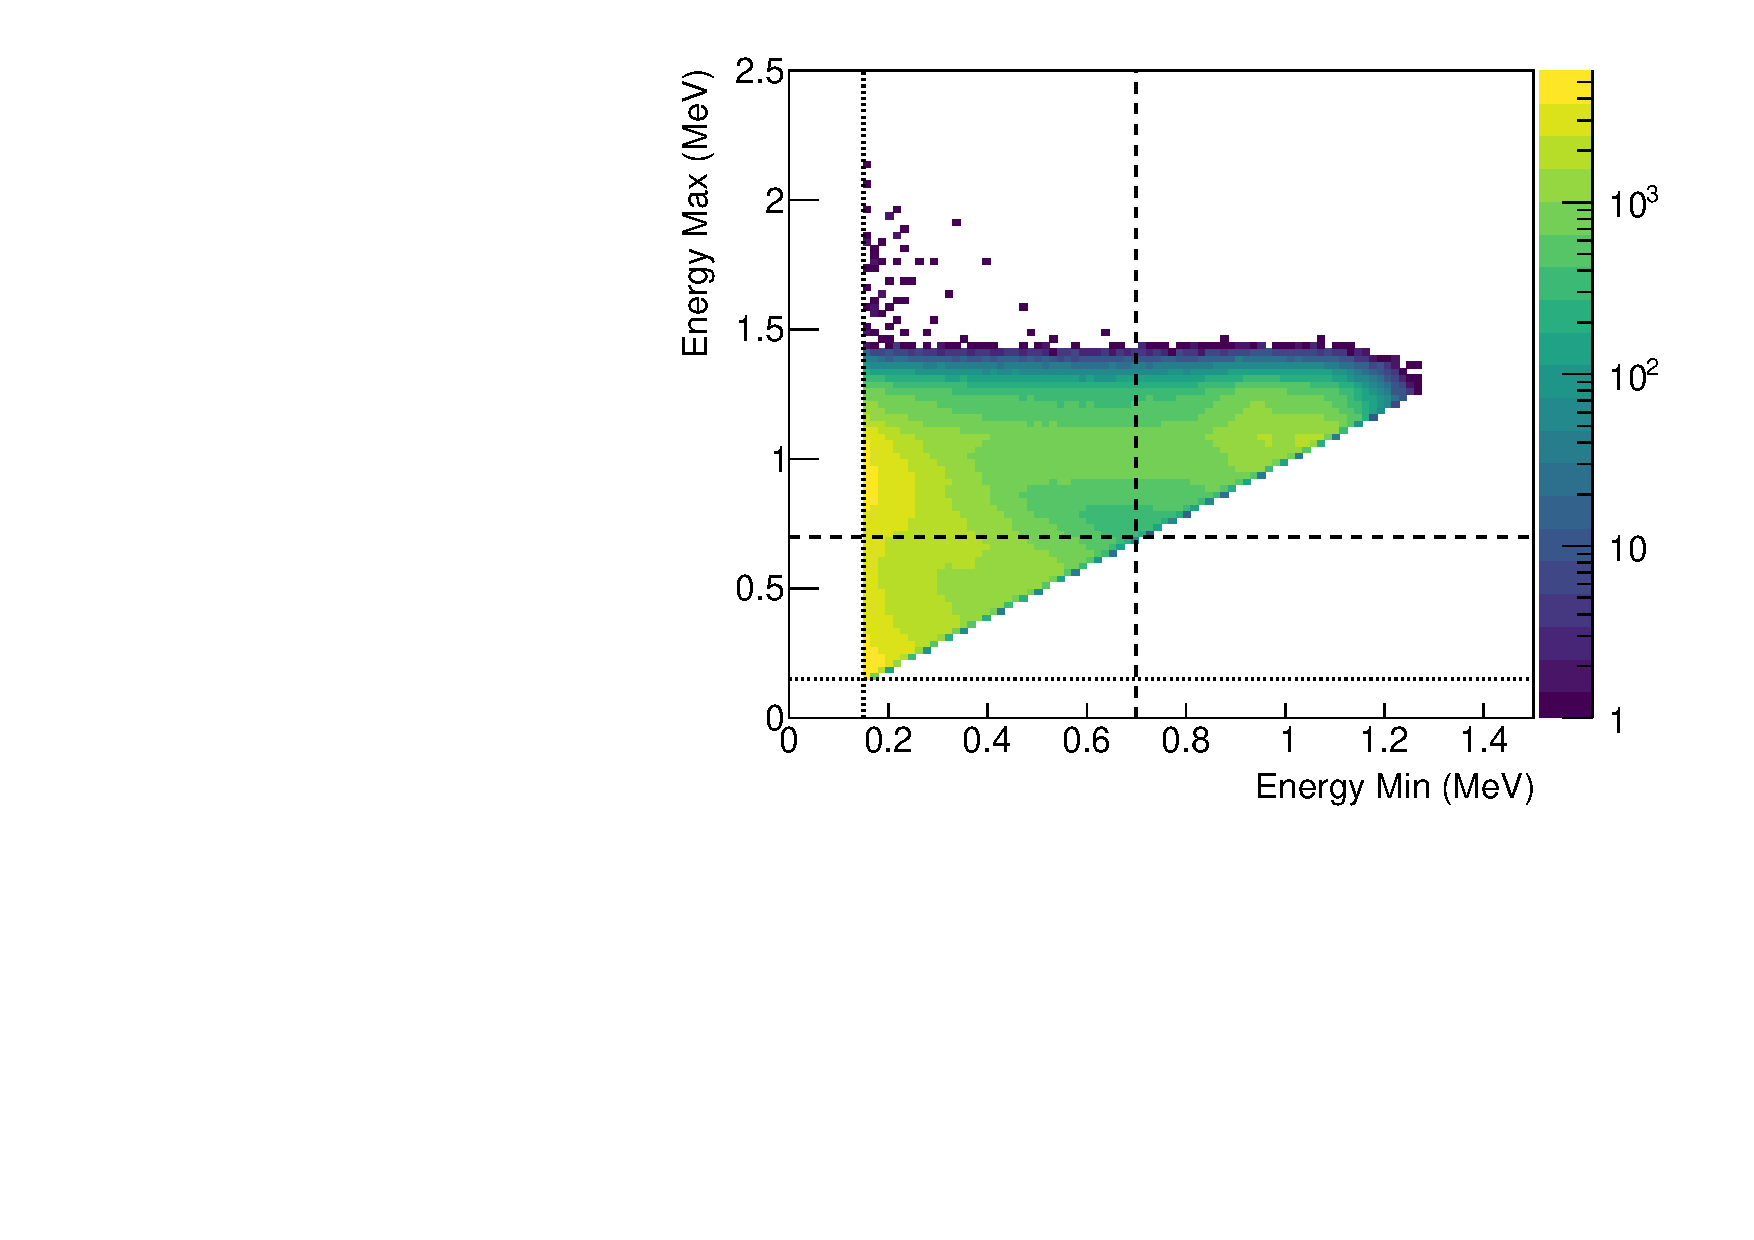
\includegraphics[width=14cm]{commissioning/fig_commissioning/Co_energy_cut.pdf}
    \caption{Maximal energy with minimal energy, for simulated Cobalt events, with source in position $5$ (see Fig.~\ref{subfig:Co_setup_wall}).
      High threshold is represented in black dotted line.
      Dashed lines materialise the individual energy selection.
      \label{fig:Co_energy_cut}}
  \end{figure}
  The high energy threshold, and the individual energy selections, are represented.
  We observe single $\gamma$ particles depositing energy successively in two optical modules, characterised by one high energy hit ($\sim 0.8$ MeV), and low energy hit ($\sim 0.2$ MeV).
  The individual energy selection allow to reject this type of events.
\item Geometrical selection:
  we want to avoid background events where one single $\gamma$ interacts in two different scintillators (by two successive Compton interactions).
  Such events occur predominantly in neighbouring scintillators.
  With a well calibrated detector, the individual energy selection would have been sufficient to prevent such events to be selected.
  But, at the time of the data-taking, the detector was not fully calibrated, and the energy for some reconstructed particle hits might be badly estimated.
  Therefore, some background events could pass this energy selection.
  Consequently, we reject events where two neighbouring optical modules detect signal in coincidence.
\end{itemize}

These four selections aim to improve the signal to background ratio.
The coincidence time selection is only applied on real data, while others are applied both on simulations and real data.
In fact, the signification of an \emph{event} is not the same for simulations as for real data: we simulate one Cobalt disintegration after another.
*a réécrire*
Each selection have an effiency
\begin{equation}
  \varepsilon = \frac{\text{Number of selected events}}{\text{Total number of events}}\,.
\end{equation}
Selection efficiencies are presented in table~\ref{tab:Co_cut_eff}.
\begin{table}[h]
  \centering

  \begin{tabular}{ l c c c }
    & Simulations & Data \\
    Trigger & $65$\% & $1.8$\% \\
    Time coincidence & - & test \\
    Individual energy & $3.4$\% & $1.2$\% \\
    Geometrical & $3.4$\% & $1.2$\% \\
  \end{tabular}

  \caption{Selection efficiencies for simulations and real data.
    \label{tab:Co_cut_eff}}
\end{table}

%% simus
%% before = 1000001 side = 917239 main = 907700 mult = 35061 event_deltat = 35061


\subsection{Background estimation}
\label{subsec:bkg_estimation}

In order to interpret the current analysis results, we aim to estimate and characterise the background detected by the SuperNEMO calorimeter, during the \Co\ data-taking time period.\\

As described previously, we aim to detect two $\gamma$'s of $1.17$ MeV and $1.33$ MeV, emitted after Cobalt disintegrations.
Therefore, we can mainly distinguish three different types of background, presented in Fig.~\ref{fig:Co_bkg}.
\begin{itemize}
\item Photons coming from the natural radioactive decay chains of $^{238}$U, $^{232}$Th and $^{40}$K isotopes.
Typically, the $2.61$ MeV-$\gamma$, from \Tl\ decay, can interact successively in two scintillators through Compton scatterings (see Fig.~\ref{subfig:Co_bkg_1}).
\item Through a double Compton interaction, a single Cobalt $\gamma$ particle can deposit energy in two scintillator blocks (see Fig.~\ref{subfig:Co_bkg_2}).
As described in Sec.~\ref{subsec:Co_datacut}, the geometrical and individual energy selections have been set up to reject these background events.
\item At the time of the data acquisition, the calorimeter was in commissioning phase, and the iron shielding was not yet installed.
Therefore, the calorimeter was not properly protected from external particles, coming from outside the detector (radioactive isotope contamination of laboratory rock).
Accidental events where two decorrelated $\gamma$ particles, can be detected in two scintillator blocks (see Fig.~\ref{subfig:Co_bkg_3}).
\end{itemize}

\begin{figure}[h]
  \centering
  \begin{subfigure}[t]{0.30\textwidth}
    \centering
    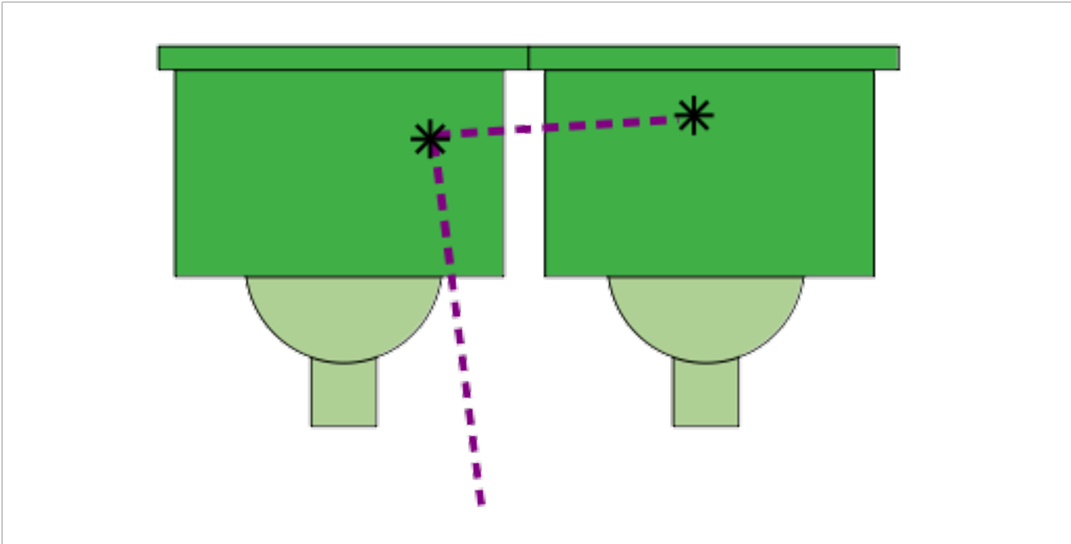
\includegraphics[height=0.50\textwidth]{commissioning/fig_commissioning/Co_bkg_1.pdf}
    \captionsetup{justification=justified}
    \caption{
      \label{subfig:Co_bkg_1}}
  \end{subfigure}
  \hfill
  \begin{subfigure}[t]{0.30\textwidth}
    \centering
    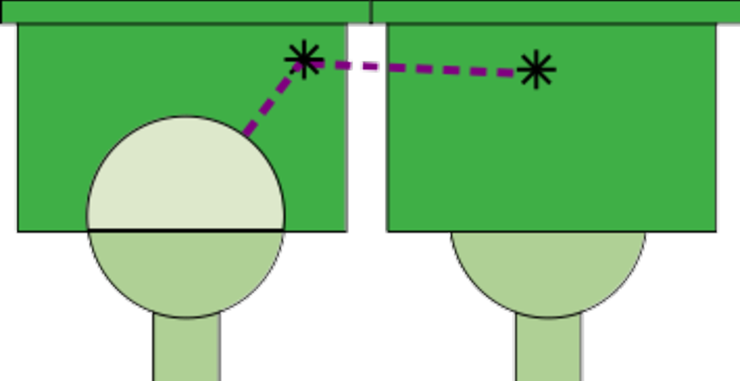
\includegraphics[height=0.50\textwidth]{commissioning/fig_commissioning/Co_bkg_2.pdf}
    \captionsetup{justification=justified}
    \caption{
      \label{subfig:Co_bkg_2}}
  \end{subfigure}
  \hfill
  \begin{subfigure}[t]{0.30\textwidth}
    \centering
    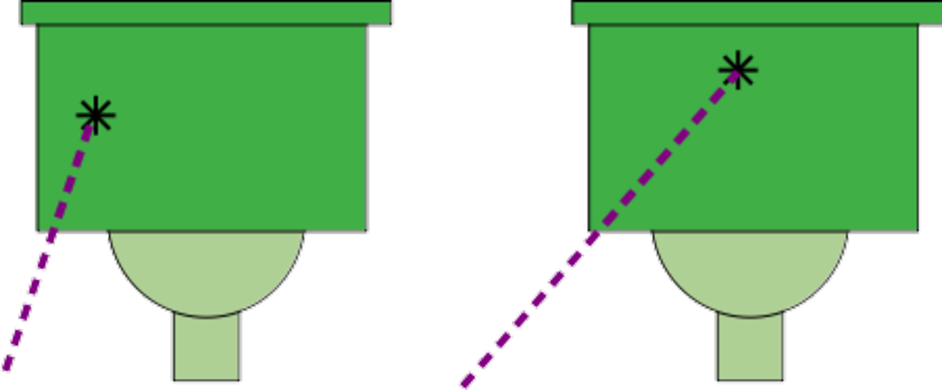
\includegraphics[height=0.50\textwidth]{commissioning/fig_commissioning/Co_bkg_3.pdf}
    \captionsetup{justification=justified}
    \caption{
      \label{subfig:Co_bkg_3}}
  \end{subfigure}
  \caption{Background types for the Cobalt study.
    Interactions of photons in scintillators are represented by black stars.
    (a) Interaction of a single Cobalt photon in two scintillators through double Compton scattering.
    (b) Interaction of a photon coming from natural radioactive isotopes contamination (PM glass...), through double Compton scattering.
    (c) Interactions of two uncorrelated photons, coming from the demonstrator outside (natural radioactivity of laboratory rock...), in two scintillator blocks
    \label{fig:Co_bkg}}
\end{figure}
All these three topologies can mimic the Cobalt two-$\gamma$'s signal.
A background acquisition, without the Cobalt calibration source, has been taken (see Sec.\ref{subsec:Co_setup}).
Unfortunately, be owing to energy calibration issues, these data are not usable.
However, estimating the amount of background received by optical blocks during the acquisition is essential to assess our results.

We aim to provide an estimation background events, considering events detected by optical modules far from the Cobalt source.
Needless to say, the data may contain signal events coming from Cobalt source, as well as background events, whose different origins are decribed above.
We choose to modelise the Cobalt data as a linear combination of signal events $s$ and background events $b$
\begin{equation}
  \hat{d}=s+b\,,
  \label{eq:estimation_data}
\end{equation}
where $s$ and $b$ are considered as uncorrelated.
The question is how to extract informations about background, using the Cobalt data acquisitions.
We remind the Cobalt source was placed at different positions behind the calorimeter wall (Fig.~\ref{subfig:Co_setup_wall}, Sec.~\ref{subsec:Co_setup}).
We aim to take advantage of those different configurations to reach our goal.
In the following, we make use of the positions $2$ and $8$ for the Cobalt source.
Therefore, depending on whether the source is in one of the two positions, some optical modules are \emph{close} to it, others are \emph{far}.
More precisely, we consider as \emph{close}, the optical modules that are separated from the source by less than 10 OMs (i.e. less than half the wall-lenght), the others being \emph{far} from it\footnote{For example, an optical module located on the left (right) of the calorimeter wall, is considered as far from (close to) the source, if the source is in position $8$.}.
Considering that, we distinguish two categories of data, $\hat{d}^{\,\text{close}}$ and $\hat{d}^{\,\text{far}}$, defined as the estimations of data events detected by an optical module when the source is close, or far to it, respectively.
Then, we precise our data modelisation with
\begin{equation}
  \hat{d}^{\,\text{close}} = b + s^{\,\text{close}}\,,
  \label{eq:estimation_data_close}
\end{equation}
where $s^{\,\text{close}}$ is the number of signal events detected by a given optical module for which $D_{\,\text{source}}<10$.
In the same way, considering $s^{\,\text{far}}$ as signal events detected by an optical module from which the source is far, we have
\begin{equation}
  \hat{d}^{\,\text{far}} = b + s^{\,\text{far}}\,.
  \label{eq:estimation_data_far}
\end{equation}
We use \Co\ simulations to gather informations on $s^{\,\text{close}}$ and $s^{\,\text{far}}$ estimations.
For this purpose, we define the coefficient $\alpha$ as
\begin{equation}
  \alpha = \tilde{s}^{\,\text{far}}/\tilde{s}^{\,\text{close}}\,,
\end{equation}
which depends on the distance $D_{\,\text{source}}$, and we find $0.05 \% < \alpha < 5 \%$ for \Co\ simulated events, meaning that the number of signal events detected by optical modules distant from the source is greatly lower than for close optical modules, for a given source position.

In order to provide a non-biased estimation of $b$, given the data model in Eq.~\eqref{eq:estimation_data_far}, we would remove $\tilde{s}^{\,\text{far}}$ (estimated through simulations) from $\hat{d}^{\,\text{far}}$ (estimated with Cobalt data acquisition).
However, qualitatively comparing data and simulations is not straightforward, especially due to detector efficiency considerations, discussed in Sec.~\ref{subsec:detector_efficiency}.
%%on voudrait avoir b=dfar, mais c'est biaisé pcq il reste signal. On pourrait enlever sfar, mais
%%c'est la merde de faire ça avec les simus
Nevertheless, we can give an order of magnitude of the amount of background events detected.
To do so, we display in Fig.~\ref{fig:Co_data_bkg} the number of calorimeter hits, after data selection, counted by each optical module, as a function of the distance to the Cobalt source.
\begin{figure}[h]
  \centering
  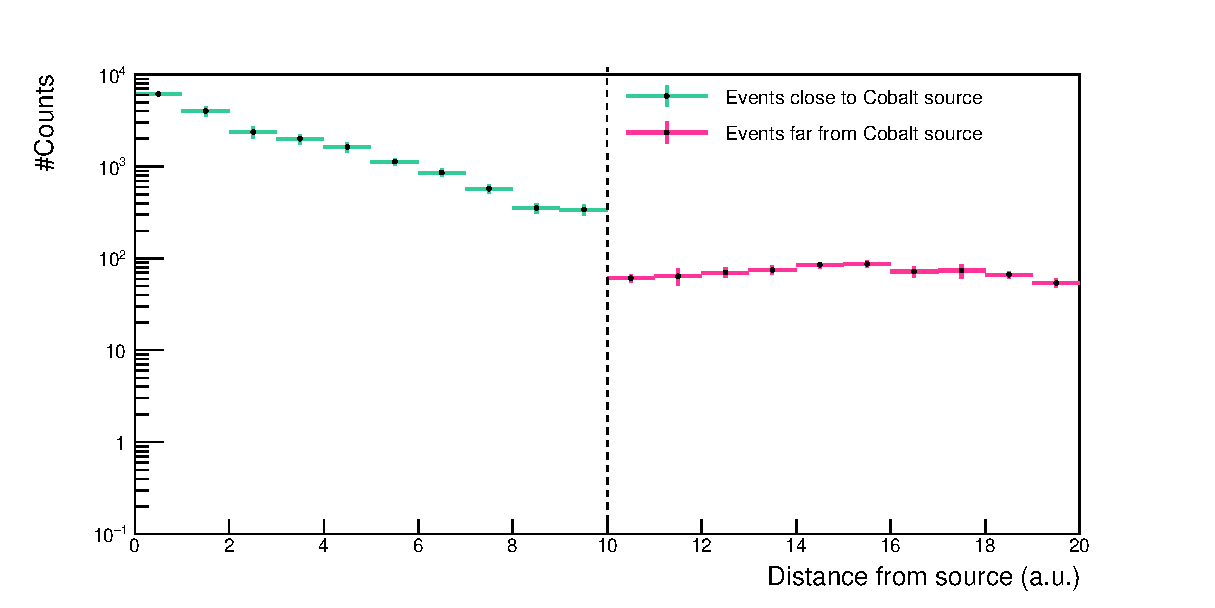
\includegraphics[width=1.1\textwidth]{commissioning/fig_commissioning/Co_data_bkg.eps}
  \caption{Number of events for pairs of OMs on the source side and on the opposite source side, for real data (green) and simulated data (red), as a function the distance to the source (in units of number of OM).
    The vertical dotted line materialises the distance limit of $10$ OMs from the source.
    \label{fig:Co_data_bkg}}
\end{figure}
The $10$ OMs limit is materialised by a vertical dashed line.
Calorimeter hits that occurred in coincidence above and below this limit are displayed both for simulated and real data.
Therefore, events where the two hits occur in two optical modules, each located in one half of the calorimeter, are not represented.
This explains the observable gap at the $10$ OMs limit level.

We first focus on simulation results.
Calorimeter hits for which $D_{\,\text{source}}<10$, represent the estimation of the amount of signal events detected close to the source, $\tilde{s}^{\,\text{close}}$.
Similarly, hits for which $D_{\,\text{source}}>10$ embed for $\tilde{s}^{\,\text{far}}$, the amount of signal events remaining for optical modules far from the calibration source site.
As expected, the number of signal Cobalt events decreases with the distance to the source.

We then compare data events with simulations.
Calorimeter hits for which $D_{\,\text{source}}<10$ materialise the number of data events estimation $\hat{d}^{\,\text{close}}$.
Apart from slight differences, discussed in Sec.~\ref{subsec:detector_efficiency}, these data events follow the same evolution as signal events with the distance to the source.
This leads us to conclude that optical modules close to the source are dominated by Cobalt signal events.
Similarly, $D_{\,\text{source}}>10$ events stand for $\hat{d}^{\,\text{far}}$.
We observe that $\tilde{s}^{\,\text{far}}/\hat{d}^{\,\text{far}} \ll 1$, which is compatible with the $\alpha$ coefficient values, being $5\%$ in the worse case, explaining the few amount of $\tilde{s}^{\,\text{far}}$ events remaining for optical modules far from the source.
Moreover, we find that the amount of $\hat{d}^{\,\text{far}}$ events is globally stable with the distance to the source.
Therefore, we assume that optical modules away from the \Co\ source by more than $10$ OMs are background dominated.
As this amount of background is comparable for all optical modules, regardless of their distance to the source, we conclude that these events are decorrelated from the Cobalt source, and come from other sources (as external $\gamma$'s).
%% donc bkg qui ne vient pas de la source
Therefore, for a $25$ minutes run, each optical module detects around $10^{2}$ external background events.
%% différence data/simus dans close : gain equalization ptetre pas dégueu sinon on verrait une diff
%% à ce niveau là. gain equalisation of optical modules, discussed in Sec.~\ref{sec:comm_energy_calibration}, could impact greatly the .

To sum up these results, calorimeter hits for optical modules close to the Cobalt calibration source are, for the most part, signal events.
Besides, hits occurring far from the source are predominantly background events.
As we moved the source in different positions, we have access to the estimation of background rate $\hat{b}$ for each optical module (when the source is far), and to the estimation of $\hat{s}$ (when the source is close).
Therefore, we can compute the signal to background ratio, as a function of the distance to the Cobalt source, displayed in Fig.~\ref{fig:Co_ratioSB}.
\begin{figure}[h]
  \centering
  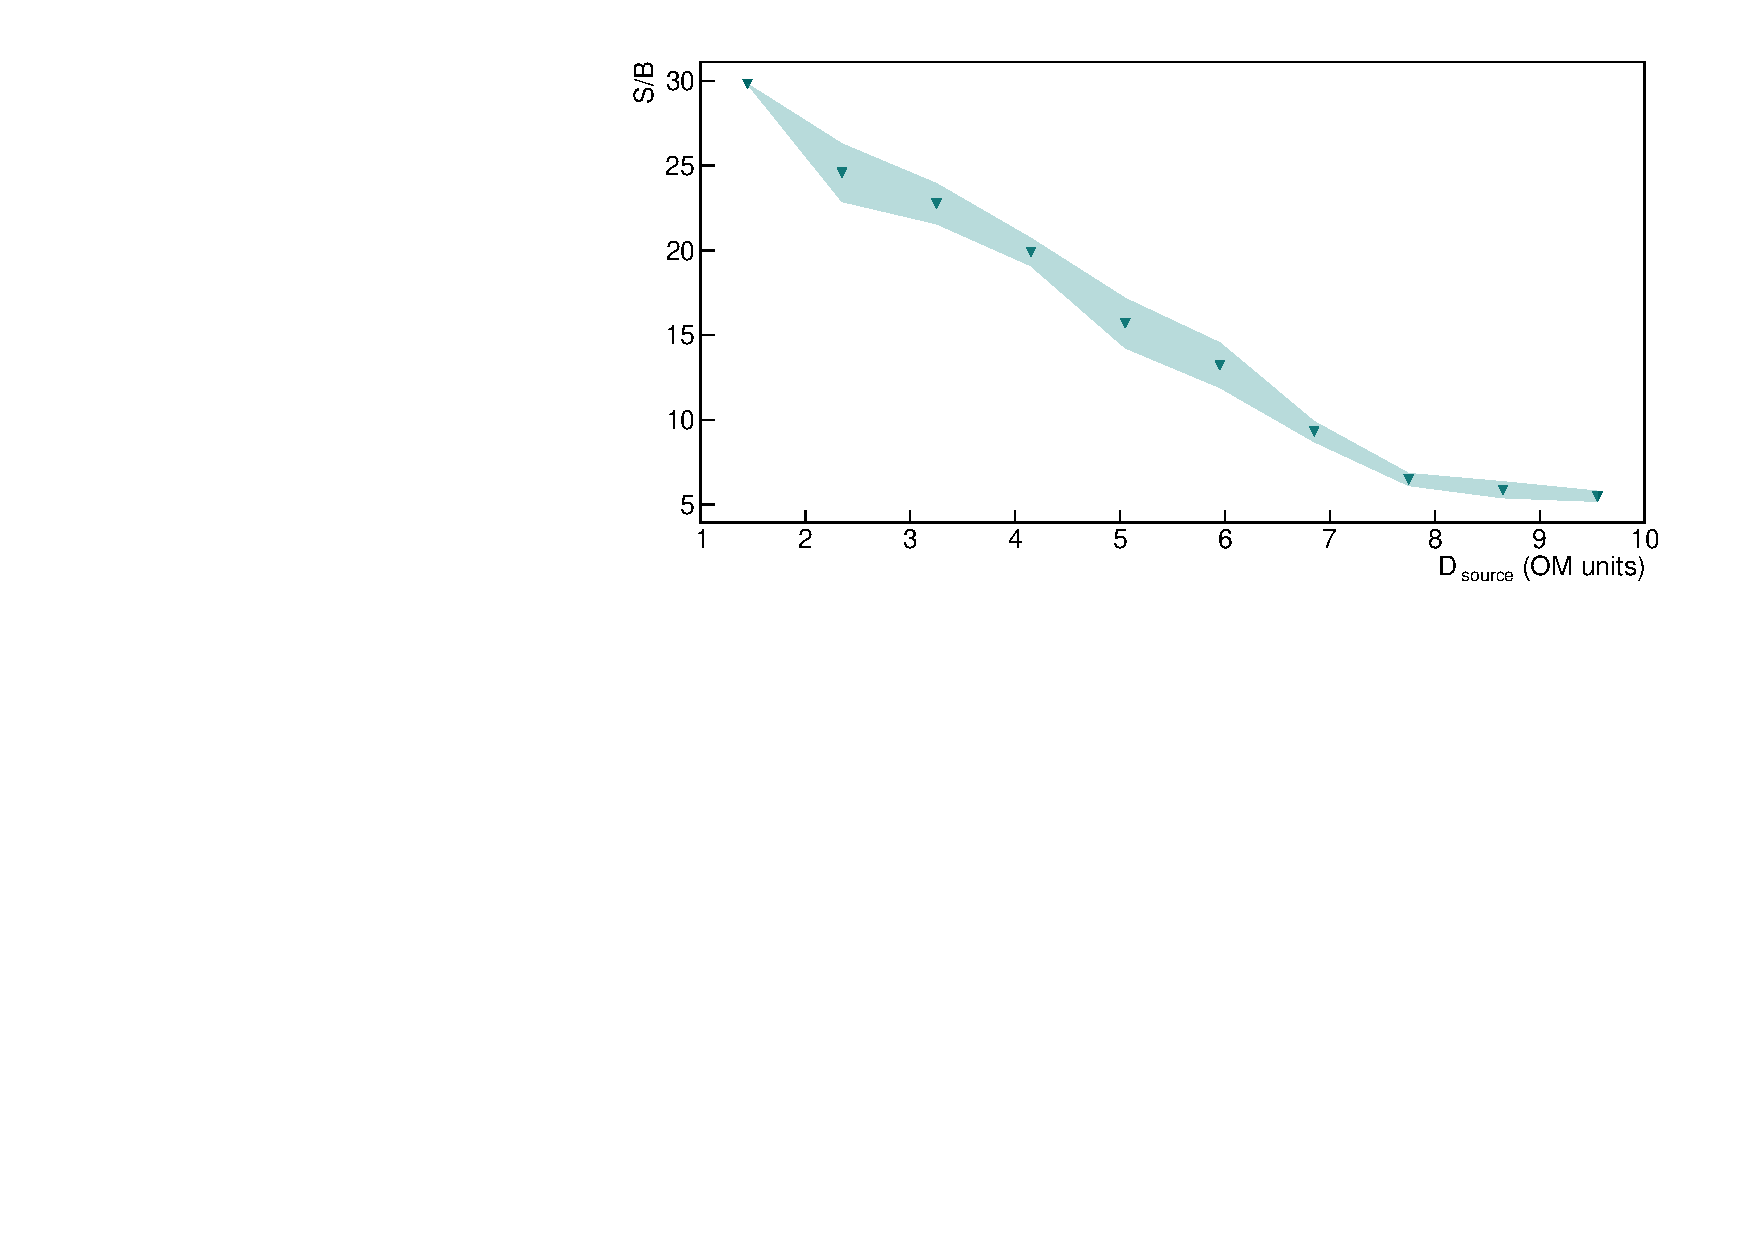
\includegraphics[width=1.1\textwidth]{commissioning/fig_commissioning/Co_ratioSB_distance.pdf}
  \caption{Signal to background ratio for each optical module, as a function of the distance to the Cobalt source.
    \label{fig:Co_ratioSB}}
\end{figure}
The number of signal events in each optical module depends on the distance to the source, which is not the case for the number of background events, explaining the decreasing of $S/B$ with $D_{\,\text{source}}$.
%% on mesure alpha et il est petit donc on peut négliger sfar dans la modélisation

To summarise, in this subsection, we gave informations on background events for the whole French wall, using data taken with the Cobalt source set at different positions.
We confirmed our assumption that the more one optical block is far from the source, the less it detects $\gamma$ particles emitted after Cobalt disintegrations, then the more the signal to background ratio decreases.
In the following, in order to properly compare simulated and real data, we give an order of magnitude of the detector efficiency during the data-taking with the Cobalt source.

%% faut dire que du coup on peut croire nos résultats quand la source est proche pour l'analyse time reso
%% aussi : Remarque : dans la suite (mesure des sigma_t), tu pourrais faire l'analyse pour les blocs
%% qui vérifient S/B > 10

%% dire qu'on peut faire ça avec d'autres runs mais que c'était pour avoir un ordre d'idée

%%Remarque : le bruit de fond peut décroitre sur les bords - ex : 2-3 dernières colonnes de PM (et
%%c'est un peu ce que tu vois sur la figure 7.8)

%% *Dire que ç'aurait été mieux de prendre un OM de ref pcq là on moyenne mais pas poss car pas de stat*
%% * finir: l'idée c'est de dire sortir un spectre en énergie data+estimation du bdf avec ce qu'on vient de faire.
%% Je vais prendre toutes les paires d'OMs possibles pour les OMs loin de la source, et tracer leur spectre en énergie en coincidence.
%% ça va me donner un histogramme binné sur l'énergie, et chaque bin aura une certaine dispersion, qui vient des différences des spectres en énergie des OMs\\



\subsection{Detector efficiency}
\label{subsec:detector_efficiency}

%% parler de la baisse d'eff du à la saturation de l'acqu
%% *A mettre quelque part:
%% the energy calibration discussed in Sec.~\ref{sec:comm_energy_calibration} was not completed, and optical modules' gains were not all aligned.*

The last step before going into detail in optical modules' timing resolution study is to determine the detector efficiency of the SuperNEMO demonstrator, during the Cobalt acquisition week.

Standing as an example, we compare real and simulated energy spectra for a given pair of optical modules detecting events in coincidence.
We provide these spectra in Fig.~\ref{fig:detector_efficiency}, where events satisfy to the four criteria described in Sec.~\ref{subsec:Co_datacut}, for the Cobalt source in position $5$.
\begin{figure}[h]
  \centering
  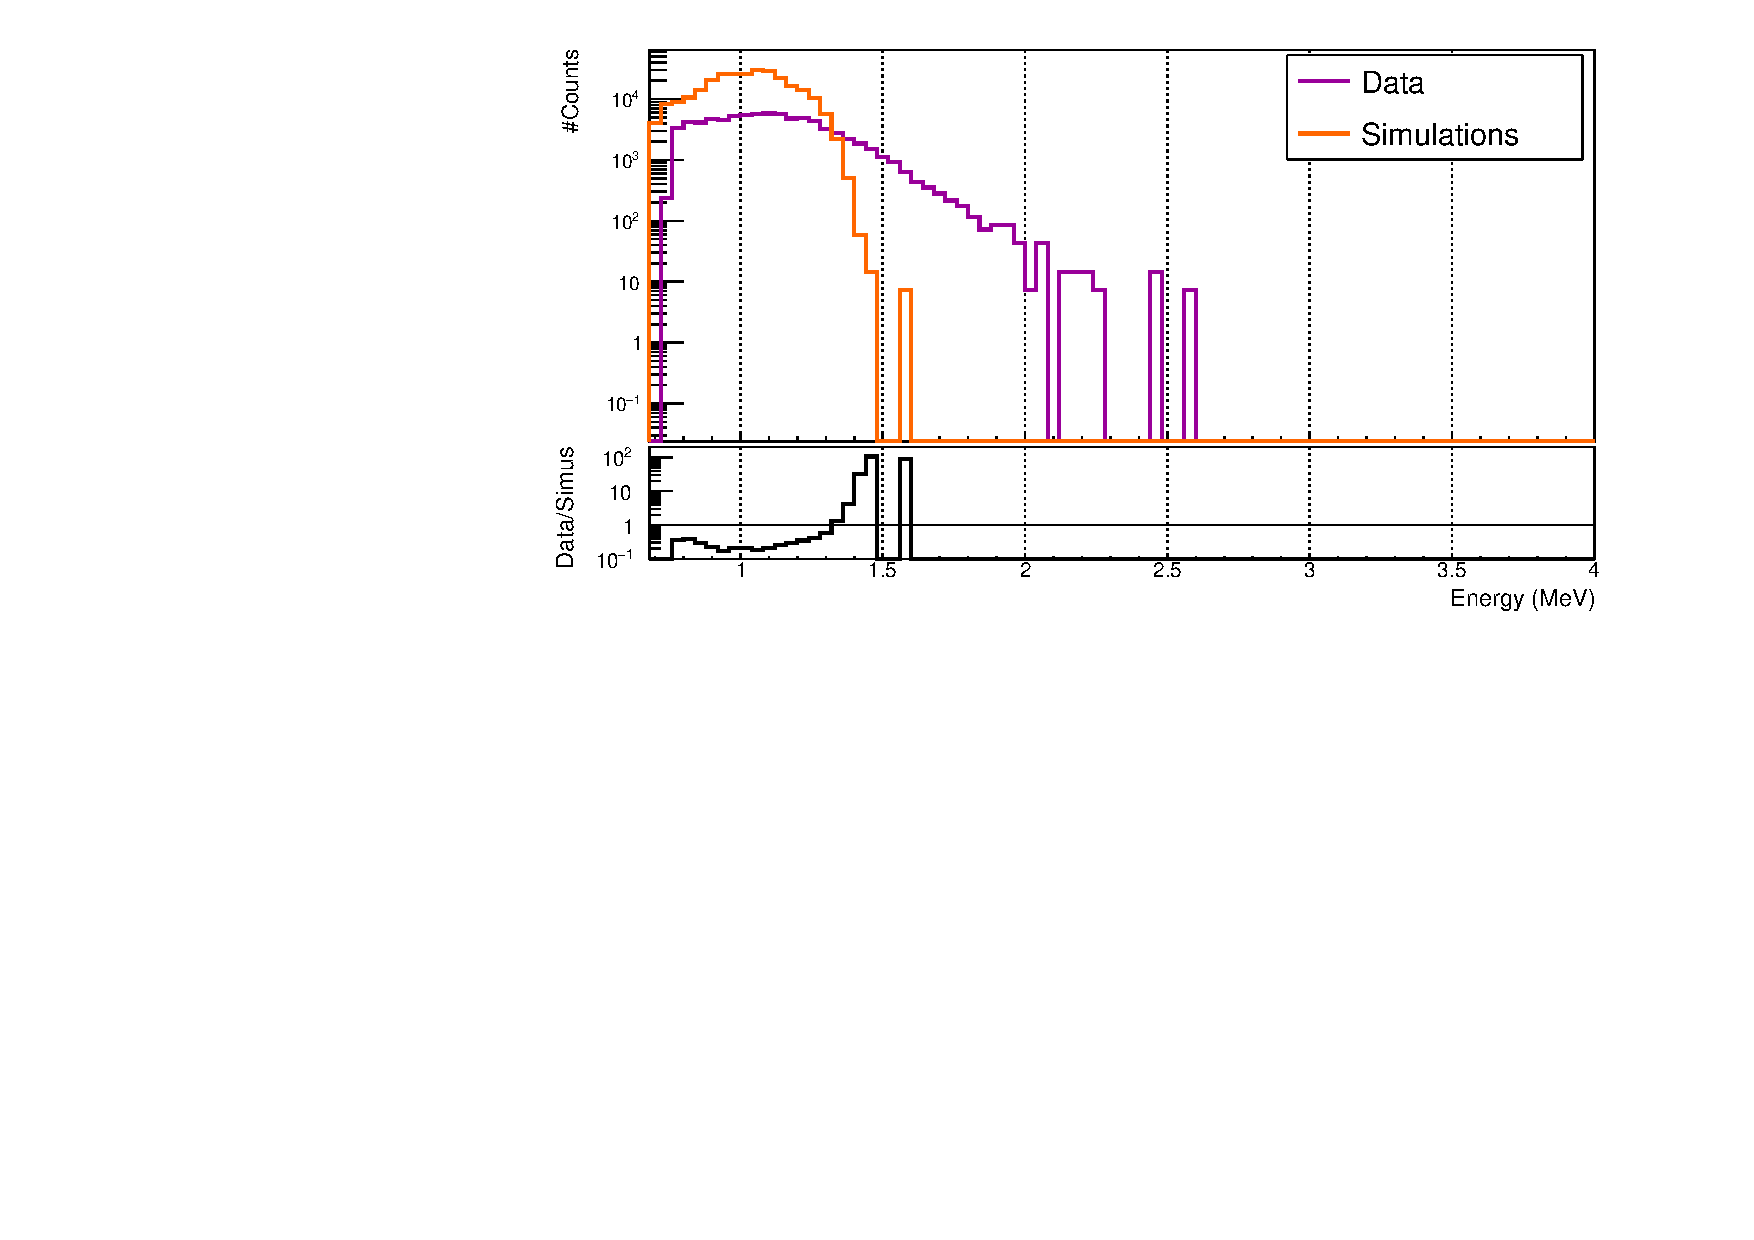
\includegraphics[width=17cm]{commissioning/fig_commissioning/Co_efficiency_detector.pdf}
  \caption{Top pad: energy spectra for simulated data (orange solid line) and real data (purple solid line) in logarithmic scale.
    Bottom pad: ratio of real data over simulated data for each bin in logarithmic scale.
    \label{fig:detector_efficiency}}
\end{figure}
The simulated data are normalised to the source activity and acquisition time.


Firstly, the energy resolution of the calorimeter blocks.
Secondly, at the time of the data taking, optical modules where not equalised in gain.
The real data energy spectrum is also characterised by a high energy part.
This may be due to external background events, which are not taken into account in the simulated data.
In Sec.~\ref{subsec:bkg_estimation} is presented a background analysis to investigate the high energy part of the energy spectrum, and better understand the data.


%% Given the amount of real and simulated events, we conclude that the detection efficiency is $29$\%.
%% Numerous parameters can affect the detection efficiency.
%% \begin{itemize}
%% \item Read out efficiency is mainly driven by
%% \end{itemize}



%% Efficiency is going to be improved.


* a finir *

\subsection{Determination of the individual timing resolution of each optical module}

%% Optical modules have been characterised before installation.
%% Performing simulations of \Co\ disintegration

\subsubsection*{Time difference distributions}

The final goal of this analysis is to determine the time resolution of optical modules, due to the scintillator time dispersion.
As displayed in Fig.~\ref{fig:Co_decay_scheme}, the two photons of Cobalt $60$ are emitted in coincidence.
The selections described in Sec.~\ref{subsec:detector_efficiency} aim to maximise the signal to background ratio, the signal being the detection of two $\gamma$'s interacting in two different optical modules.
The two $\gamma$'s, travelling at speed of light in air, reach the two optical modules at two different times.
The time of a calorimeter hit $t^{\gamma}_{i}$, describes in Fig.~\ref{fig:CFD} in Chapter~\ref{ch:commissioning}, is defined from the collected charge sampling at PM anode and received by the electronic readout.
%% We are interested in event topologies where the two $\gamma$'s of Cobalt $60$ hit two different calorimeter blocks.
We then look for topologies where two calorimeter hits occurred in a given time window of $62.5$ ns.
This coincidence time window where chosen to select the two Cobalt $\gamma$'s coincidence events, avoiding accidentals.
A first event occur in one of the scintillator of the wall, meaning the amount of charge is high enough to pass the high amplitude threshold.
In the considered coincidence time window, a second particle interacts in another scintillator.
This topologies are likely to happen for all combinations of pairs of PMs (given the distance between the two optical modules).
Therefore, we can construct a $\Delta t^{\text{pair}}$ distribution for each pair of OM, defined as the time difference between two calorimeter hits $\Delta t^{\text{pair}} = t^{\gamma}_{A} - t^{\gamma}_{B}$.
Here, one of the two optical modules, namely the $A$, is chosen as reference.

In Fig.~\ref{fig:Co_deltat} is presented an example of a $\Delta t^{\text{pair}}$ distribution, for a given pair of optical modules, both for the simulated and real data, with the Cobalt source placed at the central position behind the calorimeter wall.
%% on ne regarde des coincidences que pour paires OM sur un même mur
\begin{figure}[h]
  \centering
  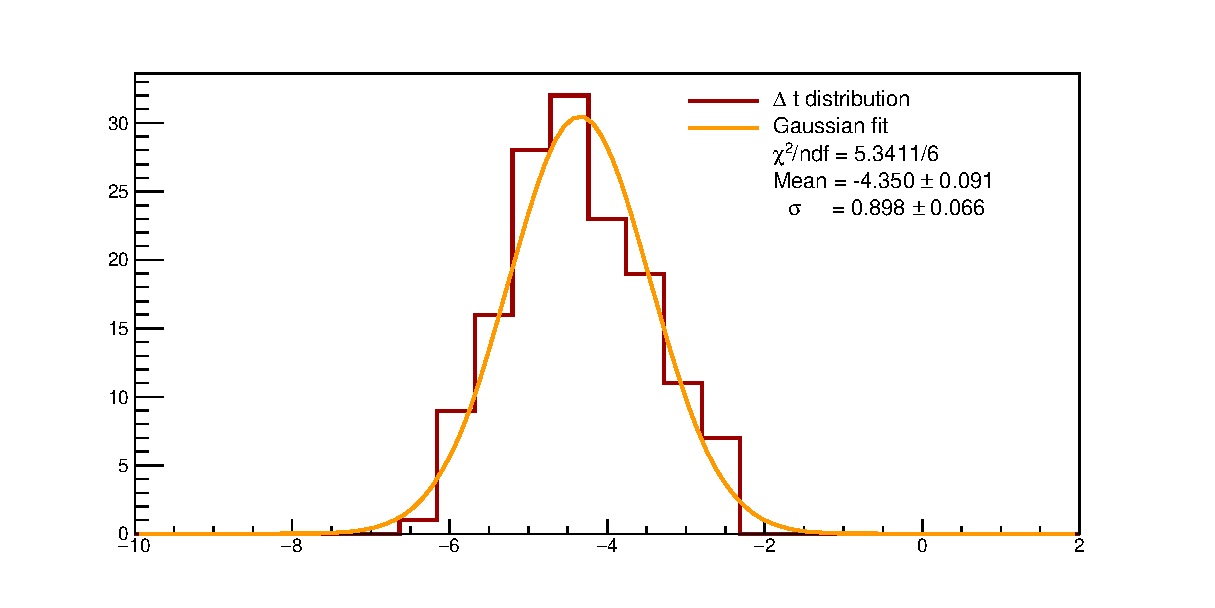
\includegraphics[width=15cm]{commissioning/fig_commissioning/Co_deltat_distrib_ex.eps}
  \caption{$\Delta t^{\text{pair}}$ distributions for real data (green solid line) and simulated data (dark red solid line).
    Two Gaussian fits (orange and blue dotted line) are displayed and fit parameters are given in the legend.
    The two distributions do not have the same mean because optical modules are not aligned in time.
    However, this does not disturb the time resolution measurements.
    \label{fig:Co_deltat}}
\end{figure}
The two distributions present different behaviours in terms of means and standard deviations.
This can be explained by two distinct reasons.

Firstly, as exposed in Sec.~\ref{subsec:OMtimeResponse}, in the framework of this study, the calorimeter part of the SuperNEMO demonstrator was considered as perfect in terms of time reconstruction, in the simulation processed.
All optical modules' time resolutions, whose main contributions are presented in Sec.~\ref{subsec:OMtimeResponse}, were set to $0$ ns.
We retrieve such a setting in the $\Delta t^{\text{pair}}$ distribution for simulated data.
As a consequence, the standard deviation, for this pair of optical module, is higher for real data than for simulated data.
Even though the case presented is just an example for a given pair of OM, we will see this is a general result for all pairs of optical modules.

Secondly, at this time, some differences remain between what is simulated and the real demonstrator performances.
In fact, as the demonstrator is in commissioning phase, some calorimeter detection characteristics are not yet included in the Falaise simulations, and affect the real data results (characterisation of optical modules' energy resolution, implementation of particle time arrival shifting due to coaxial cables...).
We observe such differences in the two distributions means: the data distribution is shifted by $3.7$ ns compared to the simulation distribution.
This result was expected: for the moment, the Falaise software does not take into account, in the reconstruction process, the time made by the electric signal to travel from a PM divider to the electronic readout, discussed in Sec.~\ref{sec:reflecto} of Chapter \ref{ch:commissioning}.
In other words, the time difference distribution for a given pair of optical module is affected by the difference of lengths of the two coaxial cables.
This is an important parameter directly affecting the mean time difference between two distinct optical modules detecting particles in coincidence.
Although simulations do not perfectly picture the full detector performances, real data and simulation can be compared, since we understand these differences.
Moreover, both the real and simulated data are affected by parameters such as the distance from the Cobalt source to the wall, or the distance between the two considered optical modules.

A $\Delta t^{\text{pair}}$ distribution exists for each pair of optical modules detecting two events in the time coincidence window.
The least square method is used to fit the distributions, which minimises the difference between the measured value and the fitted value.
A mean and a standard deviation is then defined for each pair of optical module whose fitted data has $\chi^{2}/\text{dof}<4$.
Therefore, each pair of optical module is characterised by the mean and standard deviation of its corresponding $\Delta t^{\text{pair}}$ distribution.
The standard deviation, noted as $\sigma_{t}^{\text{pair}}$ in the figure legend, corresponds to the uncertainty on time measurement for this peculiar pair of OM.
Therefore, a value of the time uncertainty $\sigma_{t}^{\text{pair}}$ can only be given for a proportion of total optical modules.

As the detector in commissioning phase, the acquisition was taken with $254$ optical modules\footnote{Three OMs are damaged on the French wall (*ref commissioning*) and three photomultipliers were not well aligned in gain at this time, and had to be removed from the analysis.}.
In this study, we only consider $8$ inches PMs, hence this analysis aims to characterise the time resolution of $214$ OMs, representing $22791$ different possible combinations of pairs.
In Fig.\ref{fig:Co_corr_sigma} are presented the $\sigma_{t}^{\text{pair}}$ values, both for simulated and real data.
\begin{figure}[h]
  \centering
  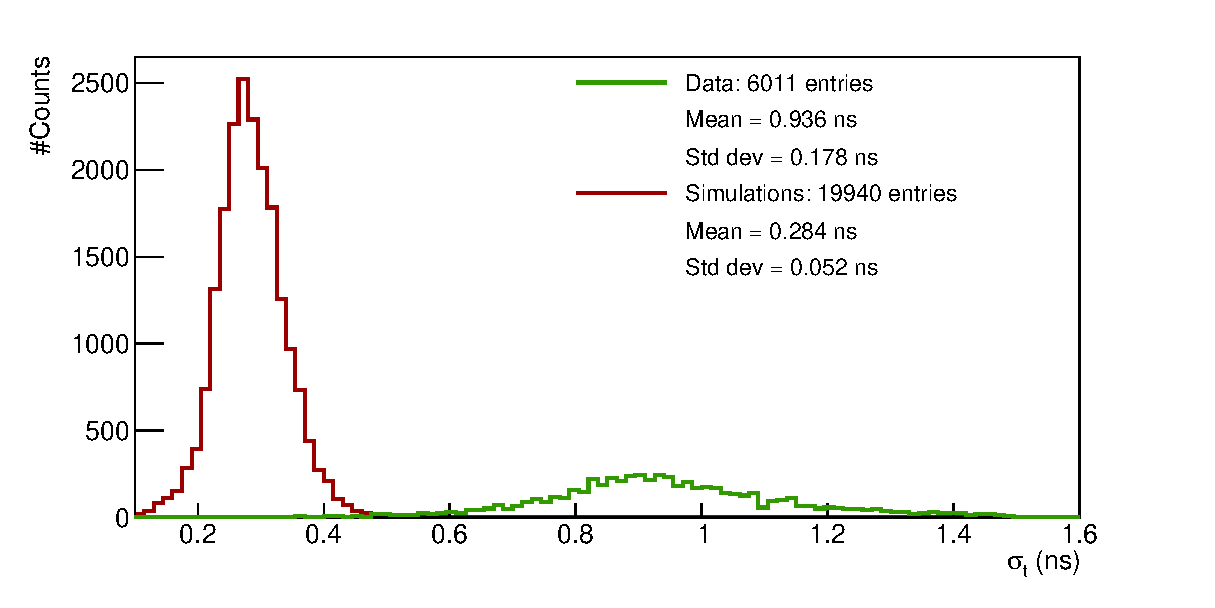
\includegraphics[width=15cm]{commissioning/fig_commissioning/Co_corr_sigma.eps}
  \caption{$\sigma_{t}^{\text{pair}}$ distribution for pairs of optical modules.
    \label{fig:Co_corr_sigma}}
\end{figure}
In the first place, we notice the mean $\sigma_{t}^{\text{pair}}$ value for simulations is lower than for real data.
As explained above, this difference is caused by the perfect calorimeter time resolution for simulations on one side, and by the detector characteristics not yet implemented in the simulation software on the other side.
This second statement is also behind the larger value of the real data distribution's standard deviation.
In fact, for the simulated case, $\Delta{t}$ distributions, of which an example is given in Fig.~\ref{fig:Co_deltat}, have comparable $\sigma_{t}^{\text{pair}}$ values, for all pairs of optical modules.
This is not the case for the real data: the $\sigma_{t}^{\text{pair}}$ value for a given pair of OM depends on the difference between the two coaxial cable lengths.
And this length difference being specific for each pair of optical module.

Moreover, we succeeded characterising $\sigma_{t}^{\text{pair}}$ values for $26$\% of pairs of optical blocks for real data, against $87$\% for simulations.
In fact, the more one optical module is from the source, the more it is background dominated.
As we explained, such a value is provided for a OM pair only if the fit of the corresponding $\Delta t^{\text{pair}}$ distribution is of high-quality.
Therefore, the optical modules for which the fit successes are the ones around the source.
This is not valid for simulations are we only have Cobalt events, and no background is simulated.

In Fig.\ref{fig:Co_sigma_distance} is displayed the number of characterised optical blocks, with the distance between the reference block and the Cobalt $60$ source, in units of block width.
\begin{figure}[h]
  \centering
  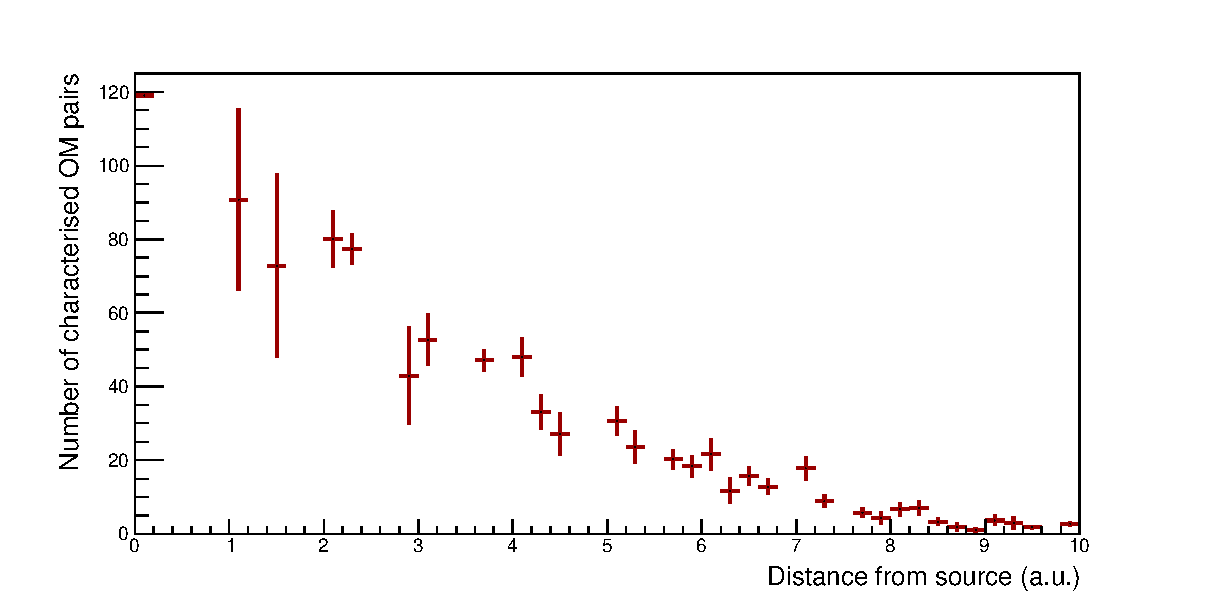
\includegraphics[width=15cm]{commissioning/fig_commissioning/Co_sigma_distance.eps}
  \caption{Number of characterised OM pairs, as a function of the distance between reference OM and source.
    \label{fig:Co_sigma_distance}}
\end{figure}
For a given distance from the source, the amount of characterised OM is lower for the real data case than for the simulated one.
This explains the different amount of characterised OMs for real and simulated data.\\

We presented results on the uncertainty on time measurement for pairs of optical module, $\sigma_{t}^{\text{pair}}$.
However, we are interesting in providing such values, independently for each optical modules.
Therefore, in the following, we present the algorithm we used to provide $\sigma_{t}^{\text{indep}}$ values.



%%fig distrib mean and sigma

\subsubsection*{Decoupling of $\sigma_{t}^{\text{pair}}$ values}

We have determined $\sigma_{t}^{\text{pair}}$ for some of the pairs of OMs on the French wall.
For example, if we take the source closest OM (OM located at the centre of the French main calorimeter wall), it has coincidence events with a certain number of other optical blocks.
Among them, $119$ different $\Delta t^{\text{pair}}$ distributions are fitted, therefore $119$ values of $\sigma_{t}^{\text{pair}}$ are stored.
And this work is done for each counting optical module taken as reference.
All following steps aim to determine the individual $\sigma_{t}^{\text{indep}}$.

We want to evaluate this value for the closest OM from the source, let us number it $0$.
We have access to the number of coincidence events this OM has with each other OMs.
We pick up the two OM that have the larger number of coincidence events with this reference OM, with their associated $\sigma_{t}^{\text{indep}}$ and mean energies.
We number them as $1$ and $2$.
Therefore, to find the value of $\sigma_{t}^{\text{indep}}$, we have to solve a set of $3$ linear equations:
\begin{align}
  (\sigma_{t}^{0,1})^{2} &= \frac{(\sigma_{t}^{0})^{2}}{\bar{E_{0}}} + \frac{(\sigma_{t}^{1})^{2}}{\bar{E_{1}}}\nonumber \\
  (\sigma_{t}^{0,2})^{2} &= \frac{(\sigma_{t}^{0})^{2}}{\bar{E_{0}}} + \frac{(\sigma_{t}^{2})^{2}}{\bar{E_{2}}}\\
  (\sigma_{t}^{1,2})^{2} &= \frac{(\sigma_{t}^{1})^{2}}{\bar{E_{1}}} + \frac{(\sigma_{t}^{2})^{2}}{\bar{E_{2}}} \nonumber\,,
  \label{eq:Co_sigma}
\end{align}
where $\sigma_{t}^{i}$ is the individual uncertainty on time measurement for the block $i$.
Solving simultaneously these equations comes down to diagonalise the matrix $S$ defined as
\begin{equation}
  S =
  \begin{pmatrix}
    1/\bar{E_{0}} & 1/\bar{E_{1}} & 0 \\
    1/\bar{E_{0}} & 0 & 1/\bar{E_{2}} \\
    0 & 1/\bar{E_{1}} & 1/\bar{E_{2}}
  \end{pmatrix}
  .
\end{equation}

We now generalise this method to all possible combinations of OM pairs for which we have informations on $\sigma_{t}^{\text{pair}}$.

\subsubsection*{Estimating the variance}



\subsection{Conclusion}
\begin{itemize}
\item il nous faut des simus bkg
\item il nous faut un run bkg
\item ça marche bien
\item il faudrait refaire une manip avec PMs alignés
  \item On aurait pu décorréler les sigmas en utilisant toutes les combinaisons possibles, mais il aurait fallu faire masse de simus pour déterminer les covariances
\end{itemize}


%%%%%%%%%%%%%%%%%%%%%%%%%%%%%%%%%%%%%%%%%%%%%%%%%%%%%%%%%%%%%%%%%%%%%%%%%%%%%%%%%%%%%%%%%%%%%%%%%%%%%%%%%%%%%%%%%%%%%%%%%%%%%%%%
\section{The Light Injection System}
\label{sec:LIS}

The SuperNEMO demonstrator is designed to have a long exposure time.
In this context, calibration systems are necessary to control and calibrate the response of the detector.
The so called \emph{Light Injection} (LI) System will monitor the stability of the calorimeter response in energy to $1$\%.
It consists in $20$ Light Emitting Diodes (LED) at $385$ nm, injecting light in each scintillator block via optical fibers.
A set of reference optical modules (PMTs coupled with scintillator blocks), receiving light from both LEDs and $^{241}$Am sources, monitors the stability of the LEDs.
A scheme of the complete LI calibration system is given in Fig.~\ref{fig:LIS_scheme}.

First LI commissioning data was taken in March 2019.



\begin{figure}[h]
  \centering
  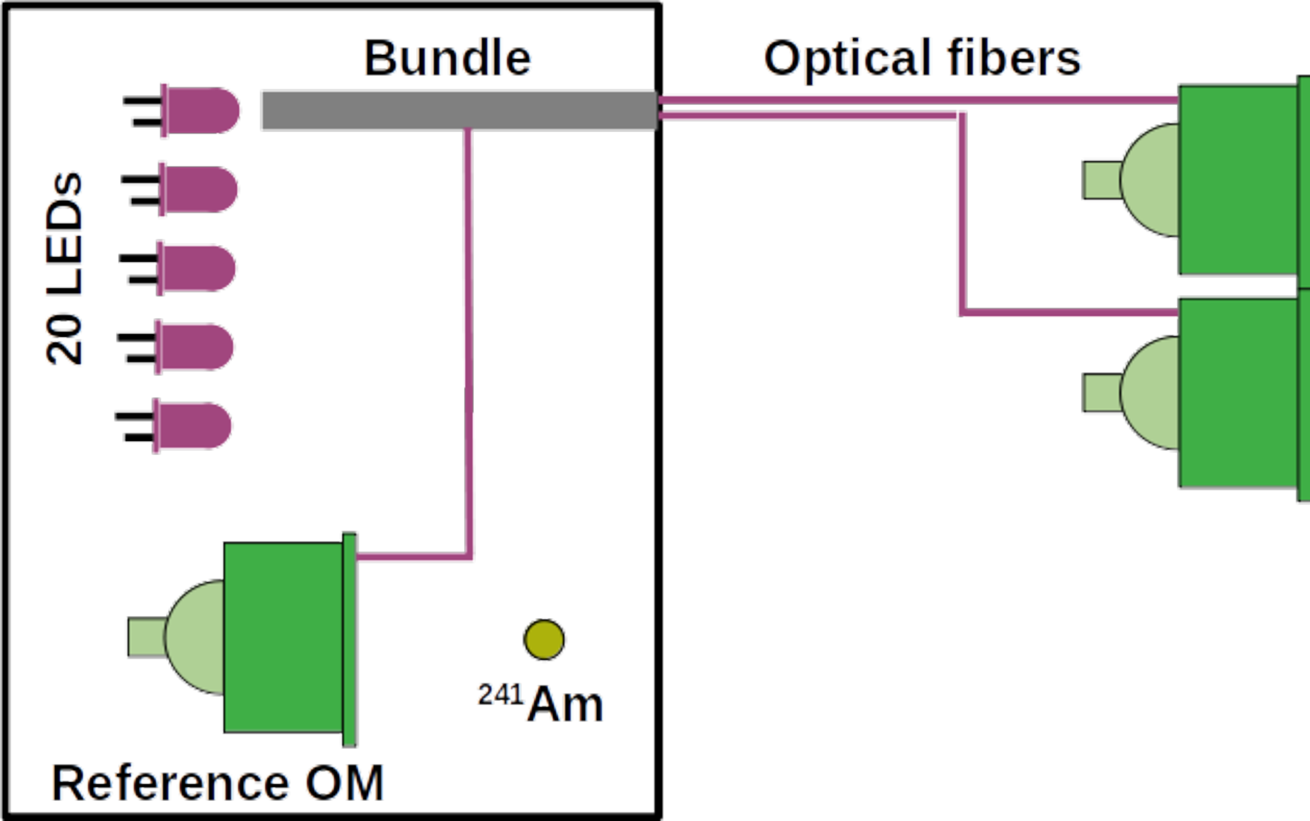
\includegraphics[width=10cm]{commissioning/fig_commissioning/LIS_scheme.pdf}
  \caption{The Light Infection (LI) calibration system is schematised.
    More than $1300$ fibers, distributed in $20$ bundles, carry the light from $20$ LEDs to each scintillator block of the demonstrator.
    Reference OMs coupled with $^{241}$Am sources monitor the LED light.
    \label{fig:LIS_scheme}}
\end{figure}

\subsection{Light injection system commissioning}


In the LI system design, the SuperNEMO demonstrator has been segmented in $10$ areas.
Each area receives light from one given LED

Primary/secondary
Each LED lights
Group LEDs/area

\begin{figure}[h]
  \centering
  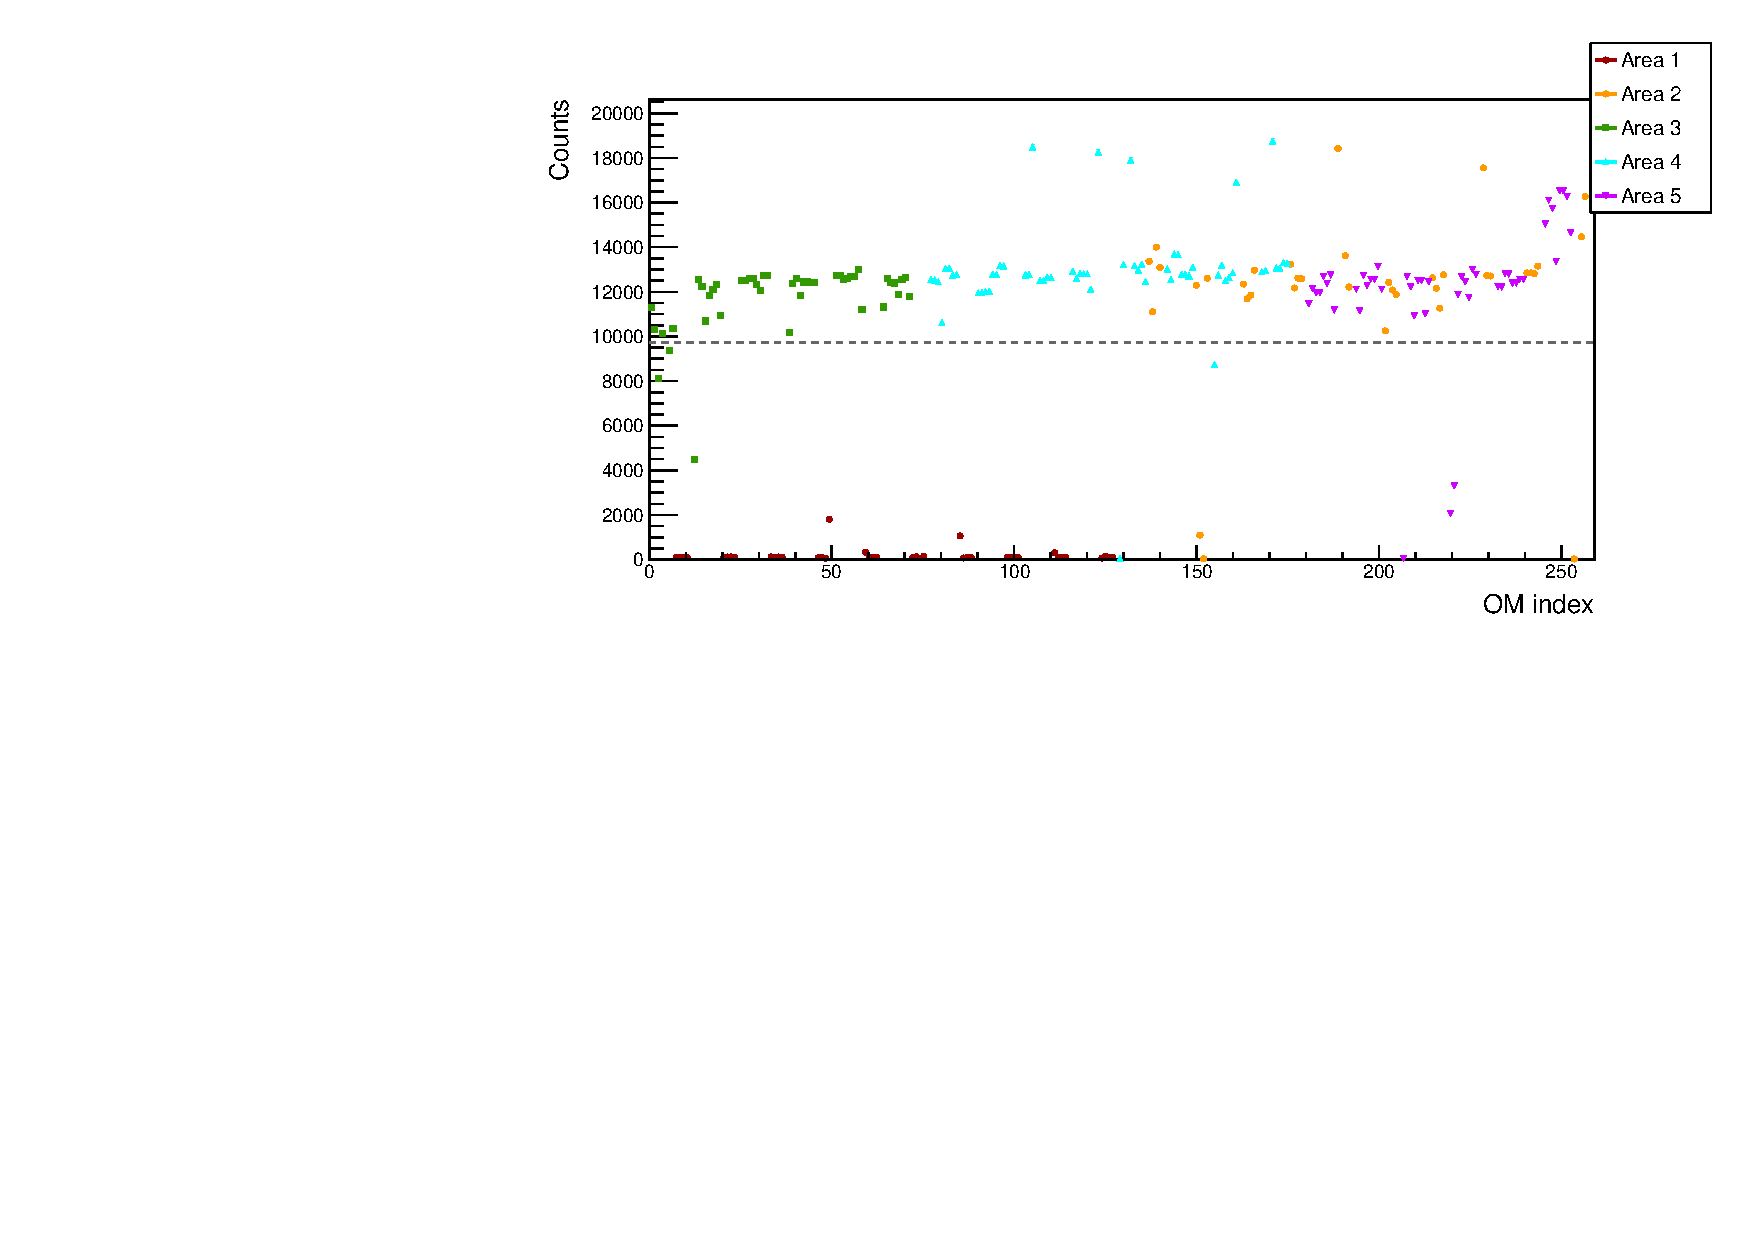
\includegraphics[width=15cm]{commissioning/fig_commissioning/LI_1d_counts.pdf}
  \caption{The number of counts is displayed for each optical module, labelled by the \emph{OM index}.
    Each coloured marker represents counting rates for one area of the detector, that is to say one group of optical modules lighted by the same LED.
    The area $1$ (dark red dots) is not receiving light from its corresponding LED.
    \label{fig:LI_counts}}
\end{figure}


\begin{figure}[h]
  \centering
  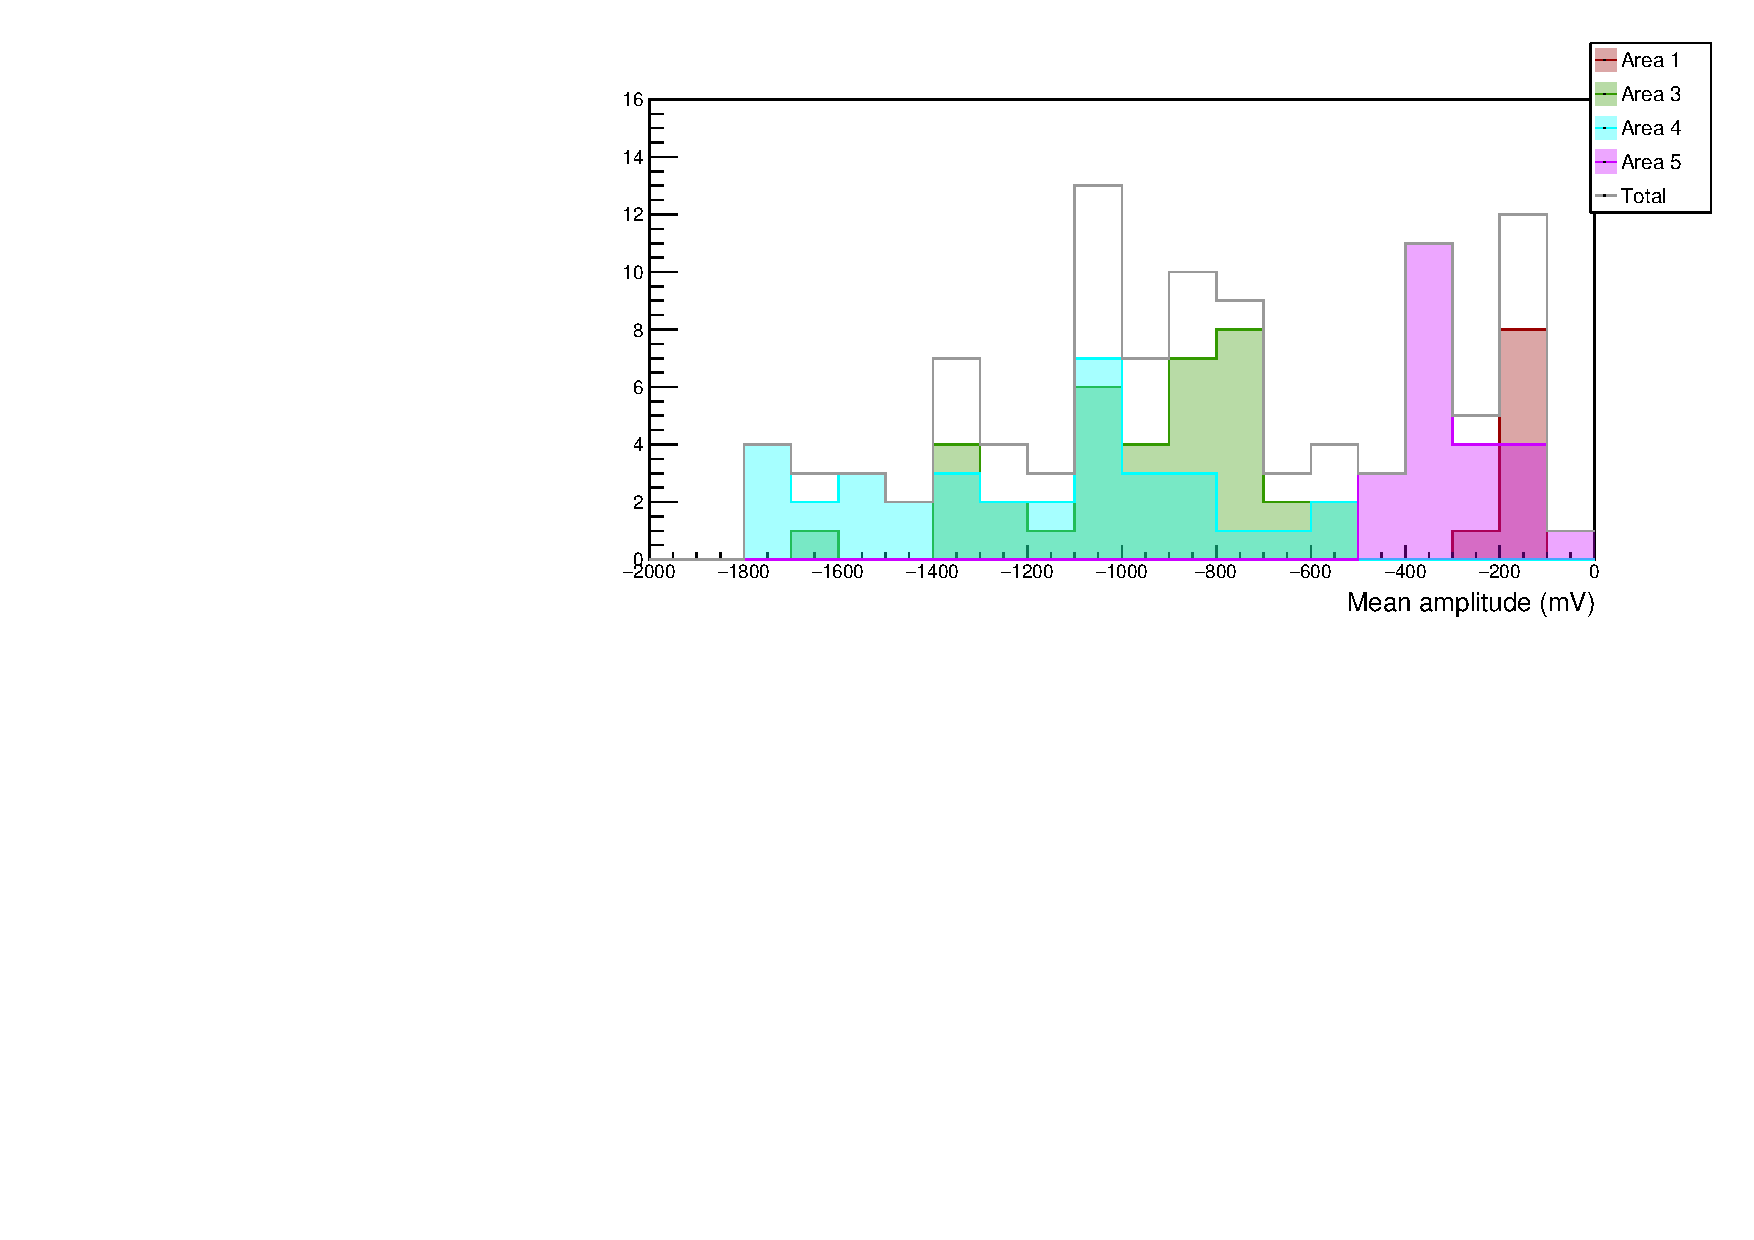
\includegraphics[width=15cm]{commissioning/fig_commissioning/LI_mean_ampl.pdf}
  \caption{The mean signal amplitude distribution for each optical module is presented.
    One colour stands for one area of the half detector.
    In Grey is the total mean amplitude distribution.
    \label{fig:LI_ampl}}
\end{figure}


\subsection{Time resolution of optical modules}



%% \begin{figure}[h]
%%   \centering
%%   \includegraphics[width=10cm]{commissioning/fig_commissioning/}
%%   \caption{
%% \label{fig:}}
%% \end{figure}



%% \begin{figure}[h]
%% \centering
%% \begin{subfigure}[t]{0.48\textwidth}
%%   \centering
%%   \includegraphics[width=1.1\textwidth]{commissioning/fig_commissioning/}
%%   \captionsetup{justification=centering}
%%   \caption{
%%     \label{subfig:}}
%% \end{subfigure}
%% \hfill
%% \begin{subfigure}[t]{0.48\textwidth}
%%   \centering
%%   \includegraphics[width=1.1\textwidth]{commissioning/fig_commissioning/}
%%   \captionsetup{justification=centering}
%%   \caption{
%%     \label{subfig:}}
%% \end{subfigure}
%% \caption{
%%   \label{fig:}}
%% \end{figure}
